\section{Obtaining Probabilities from Information on Uncertainty}
In this chapter, we propose a method for obtaining a probability distribution over the trace realizations of any uncertain process instance by exploiting the explicit description of uncertainty present in the event attributes. 
We motivate the importance of computing the probability estimates using the example process instance whose behavior graph is shown in Fig. \ref{fig: estimate motivation graph}.
The structure of the behavior graph indicates that events $e_2$ and $e_3$ have overlapping timestamps.
Additionally, event $e_4$ is indeterminate.
Thus, for $E=\{e_1,e_2,e_3,e_4\}$, the set $\mathcal{R}_e(E)$ of the correct evaluation orders contains two sequences where $e_4$ occurrs: 
$\langle e_1,e_2,e_3,e_4 \rangle$ and $\langle e_1,e_3,e_2,e_4 \rangle$, and two sequences where $e_4$ does not occurr: 
$\langle e_1,e_2,e_3 \rangle$ and $\langle e_1,e_3,e_2 \rangle$.
Since event $e_3$ might execute $b$ or $c$, whereas activity $d$ might not be executed, there are six possible traces of activities corresponding to this case (see Fig. \ref{fig: estimate motivation graph}).
%
%
%
%
%
%
\begin{figure}[h]
	\centering

	\begin{tikzpicture}[->,>=stealth',shorten >=1pt,node 						distance=2.5cm,auto,main node/.style={circle,draw,align=center}]
	%\draw [help lines] (0,0) grid (10,3);
	\node[main node,label=above: \large $a$] (A) at (3,2) {$e_1$};
	\node[main node,label=above: \large $b$] (B) at (6,3) {$e_2$};
	\node[main node,label=above: \large ${b: 0.8, c: 0.2 }$] (C) at (6,1) {$e_3$};
	\node[main node,dashed,label=above: \Large $\substack{d \\ ?:0.9, ~ !: 0.1}$] (D) at (9,2) {$e_4$};
	
	\path
	(A) edge (B)
	(A) edge (C)
	(B) edge (D)
	(C) edge (D)
	

	;
	\end{tikzpicture}
	\caption{The behavior graph of an uncertain process instance with ucnertainty type $[T]_{\mathbb{S}}[A,O]_{\mathbb{W}}$.
	The possible traces are $\langle a,b,c,d \rangle$, $\langle a,c,b,d \rangle$, $\langle a,b,b,d \rangle$, $\langle a,b,c \rangle$, $\langle a,c,b \rangle$ and $\langle a,b,b \rangle$. 
	}
	\label{fig: estimate motivation graph}
\end{figure}
%
%
%
%
%
%
%
%
%

Now suppose that the Petri net in Fig. \ref{fig: estimate motivation model} shows the normative model of the same process.
The model prescribes two possible traces: $\langle a,b,c,d \rangle$ and $\langle a,c,b,d \rangle$.
According to the model, activities $c$ and $d$ must be executed during each run.
The uncertainty information enclosing events $e_3$ and $e_4$, however, indicates that the most likely traces are the ones where activities $c$ and $d$ do not appear.
This is because $c$ is much less likely to be executed during $e_3$ than $b$, and event $e_4$ which is responsible for executing $d$, most probably did not occurr.
%
\begin{figure}
	\centering
	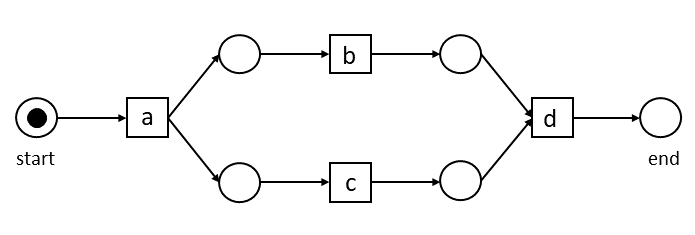
\includegraphics[width=0.8\columnwidth]{figures/estimate_motivation_model.png}
	\caption{The normative process model of the same process related to the instance from Fig. \ref{fig: estimate motivation graph}.}
	\label{fig: estimate motivation model}
	%width=1\columnwidth
\end{figure}
%
%
%
In this case, the uncertainty description of the events indicates that some traces are much more likely than others.
Moreover, it is the non-conforming traces that appear to be the most probable ones.

Before we show how one can obtain the probability estimates for all activity trace realizations, it is important to stress our assumption that the information on uncertainty related to a particular attribute in some event satisfies the following:
It is independent from the possible values of the same attribute present in other events (same attribute different events independence), and it is independent from the uncertainty information on the other attributes of the same event (same event different attributes independence).
As we will see, this assumption underlies the way the probability estimates for the activity trace realizations are obtained in the remainder of this work.
Furthermore, for any given event set of some uncertain process instance we identify its uncertainty type as we explained in Chapter \ref{chap:prelim}.
Then, we can treat all events belonging to the same instance as if they had this particular uncertainty type.
This poses no constraint since as we showed in Chapter \ref{chap:prelim}, each attribute value of another uncertainty type can be modified into an equivalent one with the desired uncertainty type.

In the remainder of this section, we always assume that for a given case $c$, we are provided with its event set $E$ and the set $\mathcal{R}_e$ containing all possible event trace realizations of case $c$.
From a process point of view, we are rather interested in the activity trace corresponding to the uncertain process instance identified by case $c$.
The set $\mathcal{R}_a$ of possible activity traces must, however, be obtained from the sets $A(s_e)$ for all $s_e \in \mathcal{R}_e$, that is, the set of activity sequences enabled by each possible event sequence (Def. \ref{def: activity trace realizations}).
From here, one can observe that the probability $\textbf{p}(s_a)$ that an activity sequence $s_a \in \mathcal{R}_a$ is indeed the activity trace of case $c$ depends from the set of all event sequences enabling it.
In the example from Fig. \ref{fig: estimate motivation graph}, both sequences $\langle e_1,e_2,e_3 \rangle$ and $\langle e_1,e_3,e_2 \rangle$ enable a common trace: $\langle a,b,b \rangle$.
The more event sequences enable a particular activity trace, the higher its likelihood.
Furthermore, for each such event sequence, one can construct a probability function $P_e(s_e)$ reflecting the likelihood of sequence $s_e$ itself and a probability function $P_a(s_a \mid s_e)$ reflecting the likelihood that the activity trace corresponding to $s_e$ is indeed $s_a$.
The value of $P_e$ is affected from the uncertainty information in timestamps and indeterminate events while the value of $P_a$ is aggregated from the uncertainty information in the activity labels.
We demonstrate some examples for this later.

From now on, we refer to the set of event trace and activity trace realizations with $\mathcal{R}_e$ and $\mathcal{R}_a$ respectively.
Furthermore, for any $s_a \in \mathcal{R}_a$ we define the set 
$ Enablers(s_a):= \{s_e \in \mathcal{R}_e \mid s_a \in A(s_e)\}$ containing the event sequences from $\mathcal{R}_e$ which might have executed activity sequence $s_a$.

Given some activity trace realization $s_a$ of some uncertain process instance and the set of its enablers, its probability is computed as following:
\begin{align*}
\textbf{p}(s_a) = \sum_{s_e \in Enablers(s_a)}P_e(s_e) \cdot P_a(s_a\mid s_e)
\end{align*} 

In the next sections, we show how $P_e$ and $P_a$ are aggregated from the uncertainty information given on event and attribute level.
For any uncertain process instance with activity trace realizations $\mathcal{R}_a$, it holds that $\sum_{s_a \in \mathcal{R}_a} \textbf{p}(s_a) = 1$, since both $P_e$ and $P_a$ are each constructed to be (independent) probability distributions.
%Also, the multiplication of the $P_e$ and $P_a$ values reflects our assumption that the uncertainty information on any attribute is independent from any uncertainty information on other attributes of the same event. 
The exact equations for $P_e$ and $P_a$ depend on the uncertainty type of the process instance in question.
For this reason, the event set of the uncertain instance must be part of the input of the probability function $\textbf{p}(\cdot)$ together with the activity trace.
For ease of notation, we omit the event set from the signature and assume the uncertainty type of the process instance in question is known or has already been determined.


\subsection{Uncertainty in Activities}
As we mentioned, $P_a(s_a \mid s_e)$ yields the probability that event sequence $s_e$ executes activity sequence $s_a$.
This value can be aggregated from the information on the uncertainty of activity labels.
If there is no uncertainty in activities, then each event has a unique activity label, that is, $\pi_a(e)$ always yields a single label from $\mathcal{U}_A$ for all $e \in s_e$.
Thus, the whole event sequence $s_e$ enables a unique activity trace $s_a$, and the value of $P_a(s_a \mid s_e)$ is trivially 1.
This is not the case whenever there is uncertainty in activities.
In that case, each event sequence $s_e \in \mathcal{R}_e$ enables every activity trace from $A(s_e)$ as defined in Def. \ref{def: cartesian activities}.

\begin{itemize}
\item
$\boldsymbol{[A]_{\mathbb{S}}}$:
If there is strong uncertainty in activities, then each event has a set of possible activity labels and no information on the likelihood of each activity.
For this reason, we assume that each activity is equally possible, which in turn implies that every sequence from $A(s_e)$ for any $s_e \in \mathcal{R}_e$ is equally possible.
Precisely, for any $s_e \in \mathcal{R}_e$ and $s_a \in A(s_e)$:
\begin{align*}
P_a(s_a \mid s_e) = \frac{1}{|A(s_e)|}.
\end{align*}

\item
$\boldsymbol{[A]_{\mathbb{W}}}$:
If there is weak uncertainty in activities, then for each event $e \in s_e$ and activity label $a \in \pi_a^{set}(e)$, the probability that $e$ executes $a$ is given by $f_A^e(a) \in F_{\mathcal{U}_A}$, where $f_A^e = \pi_a(e)$.
Again, we assume that for all $e \in s_e$, the distributions over their activity sets are independent.
Thus, for every $s_e=\langle e_1,...,e_n \rangle \in \mathcal{R}_e$ and $s_a = \langle a_1,...,a_n \rangle \in A(s_e)$, the value $P_a$ can be easily aggregated from these distributions the following way:
\begin{align*}
P_a(s_a \mid s_e) = \prod_{i=1}^{n} f_A^{e_i}(a_i) 
\end{align*}
\end{itemize}
Fig. \ref{fig: activities strong} and \ref{fig: activities weak} show the examples of a process instance with uncertainty in activities.
In the first example (Fig. \ref{fig: activities strong}) we only know the set of possible labels of events $e_2$ and $e_3$.
Here, all activity traces enabled by the same event trace are equally possible.
In the second case in Fig. \ref{fig: activities weak}, we also know the likelihood of each possible activity label of events $e_2$ and $e_3$.
These values are now taken into consideration when computing the probability that a sequence $s_e$ enables a particular activity trace $s_a \in A(s_e)$.
%
%
%
%
%
\begin{figure}[h]
\centering

	\begin{tikzpicture}[->,>=stealth',shorten >=1pt,node 						distance=2.5cm,auto,main node/.style={circle,draw,align=center}]
	%\draw [help lines] (0,0) grid (7,3);
	\node[main node,label=above: \large $a$] (A) at (1,2) {$e_1$};
	\node[main node,label=above: \large ${\{b,c\}}$] (B) at (3,3) {$e_2$};
	\node[main node,label=above: \large ${\{c,d\}}$] (C) at (5,3) {$e_3$};
	\node[main node,label=above: \large $d$] (D) at (4,1) {$e_4$};
	\node[main node,label=above: \large $e$] (E) at (7,2) {$e_5$};
	
	\path
	(A) edge (B)
	(B) edge (C)
	(A) edge (D)
	(C) edge (E)
	(D) edge (E)
	

	;
	\end{tikzpicture}
	\caption{Example of a process instance with strong uncertainty in activities. 
	Here, $\mathcal{R}_e=\{ 
	s_e^1=\langle e_1,e_2,e_3,e_4,e_5 \rangle, 
	s_e^2=\langle e_1,e_2,e_4,e_3,e_5 \rangle, 
	s_e^3=\langle e_1,e_4,e_2,e_3,e_5 \rangle \}$.
	For every $s_a \in A(s_e^1)=\{
	\langle a,b,c,d,e \rangle,
	\langle a,c,c,d,e \rangle,
	\langle a,b,d,d,e \rangle,
	\langle a,c,d,d,e \rangle\}$,
	we have $P_a(s_a \mid s_e^1) = 1/4$.	
	}
	\label{fig: activities strong}
\end{figure}
%
%
%
%
%
%
%
%
%
%
\begin{figure}[h] 
\centering

	\begin{tikzpicture}[->,>=stealth',shorten >=1pt,node 						distance=2.5cm,auto,main node/.style={circle,draw,align=center}]
	%\draw [help lines] (0,0) grid (7,3);
	\node[main node,label=above: \large $a$] (A) at (1,2) {$e_1$};
	\node[main node,label=above: \Large ${\substack{b:~0.7 \\ c:~0.3}}$] (B) at (3,3) {$e_2$};
	\node[main node,label=above: \Large ${\substack{c:~0.4 \\ d:~0.6}}$] (C) at (5,3) {$e_3$};
	\node[main node,label=above: \large $d$] (D) at (4,1) {$e_4$};
	\node[main node,label=above: \large $e$] (E) at (7,2) {$e_5$};
	
	\path
	(A) edge (B)
	(B) edge (C)
	(A) edge (D)
	(C) edge (E)
	(D) edge (E)
	

	;
	\end{tikzpicture}
	\caption{Example of a process instance with weak uncertainty in activities.
	Sequence $s_e=\langle e_1,e_2,e_3,e_4,e_5 \rangle \in \mathcal{R}_e$ is a possible event trace.
	For $s_a'=\langle a,b,d,d,e\rangle, s_a''=\langle a,c,c,d,e \rangle \in A(s_e)$, we have
	$P_a(s_a' \mid s_e)=f_A^{e_1}(a) \cdot f_A^{e_2}(b) \cdot f_A^{e_3}(d) \cdot f_A^{e_4}(d) \cdot f_A^{e_5}(e) = 1 \cdot 0,7 \cdot 0,6 \cdot 1 \cdot 1 
	= 0,42$, whereas 
	$P_a(s_a'' \mid s_e)=f_A^{e_1}(a) \cdot f_A^{e_2}(c) \cdot f_A^{e_3}(c) \cdot f_A^{e_4}(d) \cdot f_A^{e_5}(e) = 1 \cdot 0,3 \cdot 0,4 \cdot 1 \cdot 1 
	= 0,12.
	$}
	\label{fig: activities weak}
\end{figure}
%
%
%
%
%

Through the value of $P_a$, we can assess the likelihood that any given event trace executes a particular activity trace.
The next step is to assess the probability of each event trace itself.


\subsection{Timestamp Uncertainty and Indeterminate Events}

In this section, we estimate the probability of each event sequence from set $\mathcal{R}_e$.
Depending on the uncertainty in timestamps and indeterminate events, not every event ordering on event set $E$ is equally likely.
For the simple case where there is no uncertainty in timestamps and all events are determinate, there is only one possible event sequence.
Trivially, we can assign a $P_e$ value of 1 to this sequence.
In the following, we go through all uncertainty scenarios that affect the likelihood of the sequences from $\mathcal{R}_e$ for some event set $E$.

\begin{itemize}
\item
$\boldsymbol{[O]_{\mathbb{S}}}$:
Since there is no uncertainty in timestamps, all events from $E$ can be totally ordered.
The behavior graph of such process instances is always a path.
Any event from $\overline{E}$ might have happened or not, but there is no information on which is more likely.
Thus, we view each sequence $s_e$ from $\mathcal{R}_e$ as equally possible:
\begin{align*}
P_e(s_e) = \frac{1}{|\mathcal{R}_e|} = \frac{1}{2^{|\overline{E}|}}.
\end{align*}

\item
$\boldsymbol{[O]_{\mathbb{W}}}$:
Since there is no uncertainty in timestamps, all events from $E$ can be totally ordered.
For any event $\overline{e} \in \overline{E}$, the function $f_O^{\overline{e}}$ yields how likely or unlikely it is that the event really happened.
For each sequence $s_e$ from $\mathcal{R}_e$ we define:
\begin{align*}
P_e(s_e) = \prod_{\substack{\overline{e} \in \overline{E}: \\ \overline{e} \in s_e}} f_O^{\overline{e}}(!)
\prod_{\substack{\overline{e} \in \overline{E}: \\ \overline{e} \not \in s_e}} f_O^{\overline{e}}(?).
\end{align*}
Fig. \ref{fig: strong indeterminate} and \ref{fig: weak indeterminate} show two small examples for these scenarios.

%
%
%
%
%
\begin{figure}[h]
	\centering
	\begin{tikzpicture}[->,>=stealth',shorten >=1pt,node 						distance=2.5cm,auto,main node/.style={circle,draw,align=center}]
	%\draw [help lines] (0,0) grid (7,3);
	\node[main node] (A) at (1,1) {$e_1$};
	\node[main node,dashed] (B) at (3,1) {$e_2$};
	\node[main node] (C) at (5,1) {$e_3$};
	\node[main node,dashed] (D) at (7,1) {$e_4$};
	
	\path
	(A) edge (B)
	(B) edge (C)
	(C) edge (D)
	

	;
	\end{tikzpicture}
	\caption{The behavior graph of a process instance with indeterminate events.
	Here, $\overline{E} = \{e_2,e_4\}$ and there are four ($4=2^{|\overline{E}|}$) possible event traces: 
	$\langle e_1,e_2,e_3,e_4\rangle, 
	\langle e_1,e_2,e_3\rangle, 
	\langle e_1,e_3,e_4\rangle, $ and
	$\langle e_1,e_3\rangle $.
	For each of those $s_e \in \mathcal{R}_e$, we have $P_e(s_e)=1/4$.}
	\label{fig: strong indeterminate}	
\end{figure}
%
%
%
%
%
%
%
%
%
%
\begin{figure}[h]
\centering

	\begin{tikzpicture}[->,>=stealth',shorten >=1pt,node 						distance=2.5cm,auto,main node/.style={circle,draw,align=center}]
	%\draw [help lines] (0,0) grid (7,3);
	\node[main node] (A) at (1,1) {$e_1$};
	\node[main node,dashed,label=above: ${!:0.6, ~?:0.4}$] (B) at (3,1) {$e_2$};
	\node[main node] (C) at (5,1) {$e_3$};
	\node[main node,dashed,label=above: ${!:0.2, ~?:0.8}$] (D) at (7,1) {$e_4$};
	
	\path
	(A) edge (B)
	(B) edge (C)
	(C) edge (D)
	

	;
	\end{tikzpicture}
	\caption{Example of a process instance with indeterminate events $e_2$ and $e_4$, where there is information on the likelihood of their occurrence.
	Here, we have $P_e(\langle e_1,e_2,e_3,e_4\rangle)=
	f_O^{e_1}(!) \cdot f_O^{e_2}(!) \cdot f_O^{e_3}(!) \cdot f_O^{e_4}(!)
	= 1 \cdot 0,6 \cdot 1 \cdot 0,2 = 0,12$, whereas 
	$P_e(\langle e_1,e_3\rangle)=
	f_O^{e_1}(!) \cdot f_O^{e_2}(?) \cdot f_O^{e_3}(!) \cdot f_O^{e_4}(?) 		= 1 \cdot 0,4 \cdot 1 \cdot 0,8 = 0,32$.}
	\label{fig: weak indeterminate}
\end{figure}
%
%
%
%
%


\item
$\boldsymbol{[T]_{\mathbb{S}}}$:
In this scenario, all events are determinate but they might be only partially ordered.
Events with overlapping timestamps might have happened in any order and we only know the time interval for every event.
Here, one has two alternatives on how to assess the likelihood of each ordering of events. 
One can view each ordering of overlapping events as equally possible.
This leads to $P_e$ assigning probability $\frac{1}{|\mathcal{R}_e|}$ to every $s_e \in \mathcal{R}_e$.
The other alternative arises from the assumption that from a possible time interval $[t_{min}(e), t_{max}(e)]$ of an event $e$, where $t_{min}(e) < t_{max}(e)$, one can conclude that the probability that event $e$ happened at some time $t \in [t_{min(e)}, t_{max}(e)]$ is $\frac{1}{t_{max}(e) - t_{min}(e)}$.
In this case, the strong uncertainty in timestamps is viewed as a special case of weak uncertainty, in which the distributions on time intervals are always uniform.
The calculation of $P_e$ can be therefore taken from the $[T]_{\mathbb{W}}$ scenario analyzed below.
Fig. \ref{fig: strong timestamp} shows the same process instance as Fig. \ref{fig: activities strong} as an example of a process instance with strong uncertainty in timestamps, where each event is determinate.
%
%
%
%
%
\begin{figure}[h]
\centering

	\begin{tikzpicture}[->,>=stealth',shorten >=1pt,node 						distance=2.5cm,auto,main node/.style={circle,draw,align=center}]
	%\draw [help lines] (0,0) grid (7,3);
	\node[main node] (A) at (1,2) {$e_1$};
	\node[main node] (B) at (3,3) {$e_2$};
	\node[main node] (C) at (5,3) {$e_3$};
	\node[main node] (D) at (4,1) {$e_4$};
	\node[main node] (E) at (7,2) {$e_5$};
	
	\path
	(A) edge (B)
	(B) edge (C)
	(A) edge (D)
	(C) edge (E)
	(D) edge (E)
	

	;
	\end{tikzpicture}
	\caption{Behavior graph of a process instance, where there is strong uncertainty in timestamps and all events are determinate. Here, we have $\mathcal{R}_e=\{ 
	\langle e_1,e_2,e_3,e_4,e_5 \rangle, 
	\langle e_1,e_2,e_4,e_3,e_5 \rangle, 
	\langle e_1,e_4,e_2,e_3,e_5 \rangle \}$ and each sequence has probability $1/3$.}
	\label{fig: strong timestamp}
\end{figure}
%
%
%
%
%
\item
$\boldsymbol{[T]_{\mathbb{W}}}$:
In this scenario, all events are determinate but they are only partially ordered.
Events with overlapping timestamps might have happened in any order and for every event $e$, the value of $f_T^e(t)$ yields the probability that event $e$ happened on timestamp $t$.
This value is always 0 for all $t < t_{min}(e)$ and $t > t_{max}(e)$ (by definition of $t_{min}$ and $t_{max}$ in the weak uncertainty scenario).
Here, we make use of this information by making the natural assumption that a particular order between any two overlapping events is more likely if the interval of one event lies further in the future than the other one's, or if the spikes in their timestamp distributions appear in a certain order.
Moreover, since the universe of timestamps is a continuous set, there is always an infinite number of timestamp values each picked from some time interval, such that their odering induces the same ordering of the corresponding events.
For this reason, the value of $P_e$ is assessed as precisely as possible by using integrals.
For a sequence $s_e=\langle e_1,...,e_n \rangle \in \mathcal{R}_e$, let $a_i:=t_{min}(e_i)$ and $b_i:=t_{max}(e_i)$ for all $1 \leq i \leq n$.
Then, we define:
\begin{align*}
I(s_e) &= \int_{a_1}^{min\{b_1,...,b_n\}} f_T^{e_1}(x_1)
\int_{max\{a_2,x_1\}}^{min\{b_2,...,b_n\}} f_T^{e_2}(x_2)
\cdot \cdot \cdot \\
&
\int_{max\{a_i,x_{i-1}\}}^{min\{b_i,...,b_n\}} f_T^{e_i}(x_i)
\cdot \cdot \cdot 
\int_{max\{a_n,x_{n-1}\}}^{b_n} f_T^{e_n}(x_n) ~
d_{x_n} ... d_{x_1} \\
&=
\int_{a_1}^{min\{b_1,...,b_n\}} 
\int_{max\{a_2,x_1\}}^{min\{b_2,...,b_n\}} 
\cdot \cdot \cdot 
\int_{max\{a_i,x_{i-1}\}}^{min\{b_i,...,b_n\}} 
\cdot \cdot \cdot 
\int_{max\{a_n,x_{n-1}\}}^{b_n} \\
&
\prod_{i=1}^{n} f_T^{e_i}(x_i) ~
d_{x_n} ... d_{x_1}.
\end{align*}

Note that the value of $I(s_e)$ sums the probabilities of all timestamp values $x_1,...,x_n$ for events $e_1,...,e_n$, where the events have happened in the order given by $s_e$, that is: $x_1 \leq ... \leq x_n$.
For the timestamps to satisfy the inequalities $x_1 \leq  ...  \leq x_n$, where each $x_i$ yields some possible timestamp of event $e_i$, each $e_i$ can only start after event $e_{i-1}$ has finished (except $e_1$ which can start at $a_1$).
Thus, the minimal possible value for $x_i$ is $max\{a_i,x_{i-1}\}$.
Also, event $e_i$ has to finish early enough so that the rest of the future events can still happen.
Therefore the maximal possible value for $x_i$ is $min\{b_i,...,b_n\}$.
Note that one can calculate the value of $I$ for any possible ordering from $\mathcal{S}_E$.
However, $I(s_e)=0$ if $s_e \not \in \mathcal{R}_e$.
In this scenario, we set $P_e(s_e)= I(s_e)$ for all $s_e \in \mathcal{R}_e$.

The integral values for the possible event orderings were computed in Python using the \texttt{scipy.integrate.nquad} method.
We implemented a method\footnote{\url{https://github.com/biankabakullari/UncertainLogProbabilities/tree/master/code/Integrals}} which enables generating events with a corresponding probability density function over its possible timestamp range, which can be a uniform or a normal distribution.
The generated pdfs are then automatically ordered in an arguments' list, which is then fed to the \texttt{nquad} method of \texttt{scipy}. 
%
%
%
\begin{table}[h]
\caption{Example of an event set with weak uncertainty in timestamps, where the distributions are all uniform over the possible time intervals.}
	\centering
	\begin{tabular}{ccc}
		\textbf{Case ID} & \textbf{Event ID} & \textbf{Timestamp} \\ \hline
	%\multicolumn{1}{c}{\cellcolor{black!30}\textbf{Case ID}} & 
  %\multicolumn{1}{c}{\cellcolor{black!30}\textbf{Event ID}} &
  %\multicolumn{1}{c}{\cellcolor{black!30}\textbf{Timestamp}}
  %\\\hline
	\multicolumn{1}{|c|}{2133} & 
	\multicolumn{1}{|c|}{$e_1$} &
  	\multicolumn{1}{c|}{\begin{tabular}[c]{@{}c@{}} $U$(11-12-2020 12:00, 11-12-2020 14:00) \end{tabular}} 
\\ \hline
	\multicolumn{1}{|c|}{2133} & 
	\multicolumn{1}{|c|}{$e_2$} &
	\multicolumn{1}{c|}{\begin{tabular}[c]{@{}c@{}}$U$(11-12-2020 15:00, 11-12-2020 17:00)\end{tabular}}                                                                                        \\ \hline
	\multicolumn{1}{|c|}{2133} & 
	\multicolumn{1}{|c|}{$e_3$} &
    \multicolumn{1}{c|}{\begin{tabular}[c]{@{}c@{}}$U$(11-12-2020 18:00, 11-12-2020 20:00)\end{tabular}}                                                                                        \\ \hline
	\multicolumn{1}{|c|}{2133} & 
	\multicolumn{1}{|c|}{$e_4$} &
	\multicolumn{1}{c|}{\begin{tabular}[c]{@{}c@{}}$U$(11-12-2020 16:00, 11-12-2020 19:00)\end{tabular}}                                                                                          \\ \hline
	\multicolumn{1}{|c|}{2133} & 
	\multicolumn{1}{|c|}{$e_5$} &
    \multicolumn{1}{c|}{\begin{tabular}[c]{@{}c@{}}$U$(11-12-2020 20:00, 11-12-2020 21:00) \end{tabular}}                                                                                     \\ \hline
		
	\end{tabular}
	\label{table: weak timestamps}
\end{table} 
%
%
%

To illustrate this with an example, consider the event set shown in Table \ref{table: weak timestamps}.
Each of the events has a possible time interval and the probability distribution on each interval follows a uniform one.
The distribution of the events in time is nicely visualized in the Gantt chart in Fig. \ref{fig: gantt}. 
%
%
%
\begin{figure}
	\centering
	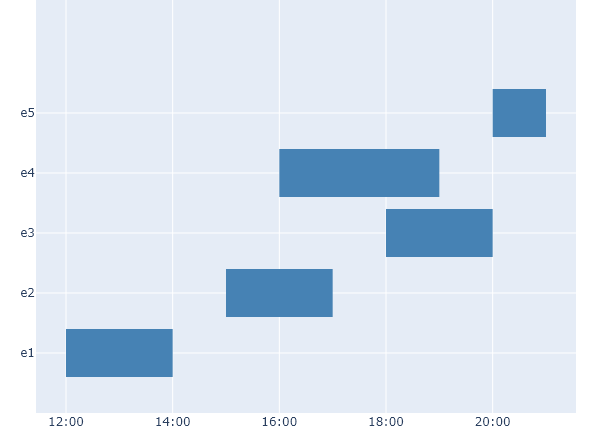
\includegraphics[width=0.8\columnwidth]{figures/gantt_thesis.png}
	\caption{A Gantt diagramm for the events of the uncertain process instance from Table \ref{table: weak timestamps}.
	Each horizontal blue bar visualizes the interval of possible timestamps of the corresponding uncertain event.}
	\label{fig: gantt}
	%width=1\columnwidth
\end{figure}
%
%
%
The behavior graph of this event set is the same as the one in Fig. \ref{fig: strong timestamp}.
Whether the uncertainty in timestamps is weak or strong does not affect the behavior graph, since the latter only captures which events overlap with each other.
As we will see in this example, however, weak uncertainty in timestamps may lead to a probability distribution over the possible event sequences that is much different from a uniform distribution.
A uniform distribution is what we assume when we have strong uncertainty in timestamps and make the decision to consider all event sequences equally likely.

Fig. \ref{fig: weak timestamp} visualizes the behavior graph for the event set together with their possible time intervals.
Note that here we have mapped the set of timestamps to a set of numbers.
This is an equivalent transformation regarding the calculation of the probabilities from $I$, since they are only affected from the relative time distances between the lower and upper bounds of the overlapping time intervals.
%
%
%
\begin{figure}[h] 
\centering

	\begin{tikzpicture}[->,>=stealth',shorten >=1pt,node 						distance=2.5cm,auto,main node/.style={circle,draw,align=center}]
	%\draw [help lines] (0,0) grid (7,3);
	\node[main node,label=above:  {$[0,2]$}] (A) at (1,2) {$e_1$};
	\node[main node,label=above:  {$[3,5]$}] (B) at (3,3) {$e_2$};
	\node[main node,label=above:  {$[6,8]$}] (C) at (5,3) {$e_3$};
	\node[main node,label=above:  {$[4,7]$}] (D) at (4,1) {$e_4$};
	\node[main node,label=above:  {$[8,9]$}] (E) at (7,2) {$e_5$};
	
	\path
	(A) edge (B)
	(B) edge (C)
	(A) edge (D)
	(C) edge (E)
	(D) edge (E)
	

	;
	\end{tikzpicture}
	\noindent
	\caption{ Behavior graph of event set from Table \ref{table: weak timestamps}, where the extremes of the time intervals are mapped to a set of numbers.
	}
	\label{fig: weak timestamp}
\end{figure}
%
%
As we already saw in the previous example, for this case the set of possible event sequences is $\mathcal{R}_e = \{
\langle e_1,e_2,e_3,e_4,e_5\rangle,
\langle e_1,e_2,e_4,e_3,e_5\rangle,
\langle e_1,e_4,e_2,e_3,e_5\rangle
\}$.
By computing the values of the integrals in $I$ as defined, we obtain  $P_e(\langle e_1,e_2,e_3,e_4,e_5\rangle) = P_e(\langle e_1,e_4,e_2,e_3,e_5 \rangle) \simeq 0.0833$,
while the second sequence is highly more likely with $P_e(\langle e_1,e_2,e_4,e_3,e_5 \rangle) \simeq 0.8333$.
The variance in the probability estimates for the three possible event traces is not surprising since according to the Gantt chart in Fig. \ref{fig: gantt}, the trace where event $e_4$ happens between $e_2$ and $e_3$ seems the most likely one. 

%
%
%
Note that the value of $I$ is 0 as soon as one of the events has a certain timestamp as a result of the lower and upper bound of the integral having the same value\footnote{Whenever we have certain timestamps, to avoid the integral taking value 0 for every ordering, we can also change the $t_{max}$ value into $t_{max}+\varepsilon$, where $\varepsilon > 0$ is a very small value, e.g. $10^{-10}$.}.
\definecolor{mygray}{gray}{0.3}
%\textcolor{mygray}{
However, the equation for computing the integral can be modified to also consider certain timestamps. 
%The integrals in this case go only over the events with uncertain timestamps, while the certain timestamps affect the lower and upper bounds.
The intuition is the following: The timestamp has more than one possible value only for the events with uncertainty in timestamps.
For this reason, we do not need to use a variable $x$ in the interval equation for the events with certain timestamps, since its value is fixed.
For a given event sequence, we construct the equation just as before, but we exclude the events with certain timestamps.
The positions of the events with certain timestamps in the sequence indicate, however, when the other events are allowed to start and end, thereby affecting the lower and upper bounds of the integrals.
Each event having a variable in the integral has to satisfy an additional condition:
it can only happen both after the last certain event appearing before it in the sequence, and before the first certain event appearing after it in the sequence.
In the following we formalize this idea.\\
For a given event set $E$ of size $n$, let 
$E^{CT} = \{e \in E \mid t_{min}(e) = t_{max}(e)\}$
be the set of events of $E$ with a certain timestamp.
Let $CT = \{t_{min}(e) \mid e \in E^{CT}\}$ be the set of the certain timestamps of events in $E^{CT}$.
Suppose $s_e=\langle e_1,...,e_n \rangle \in \mathcal{R}_e$ is a possible event ordering for which we want to estimate $I(s_e)$.
For every event $e_j \in s$ with $j \in \{1,...,n\}$ such that $e_j \in E \setminus E_{CT}$, we define the following sets:
\begin{align*}
before(e_j) &= \{t \in CT \mid t=t_{min}(e_i) \text{ for some } e_i \in s_e, ~ s.t. ~ e_i \in E_{CT} \wedge i<j\} \\
after(e_j) &= \{t \in CT \mid t=t_{min}(e_i) \text{ for some } e_i \in s_e, ~ s.t. ~ e_i \in E_{CT} \wedge i>j\}.
\end{align*}
From these sets we can obtain two values: 
\begin{align*}
ts^*_{before}(e_j) &= \begin{cases}
	max\{t \in before(e_j)\} & \mbox{if} \; before(e_j) \neq \emptyset,\\
	t_{min}(e_j) & \mbox{otherwise}, \; 
	\end{cases} \\
	%\text{ and } \\
ts^*_{after}(e_j) &= \begin{cases}
	min\{t \in after(e_j)\} & \mbox{if} \; after(e_j) \neq \emptyset,\\
	t_{max}(e_j) & \mbox{otherwise}. \; 
	\end{cases} \\
\end{align*}
Here, $ts^*_{before}(e_j)$ yields the certain timestamp of the last event from $E_{CT}$ that appears before $e_j$ in the ordering, whereas $ts^*_{after}(e_j)$ yields the certain timestamp of the first event from $E_{CT}$ that appears after $e_j$ in the ordering.\\
To obtain the probability of having a particular event ordering $s_e \in \mathcal{R}_e$, we first obtain the subsequence $s_e'\sqsubseteq s_e$ such that $s_e' = s_e \downharpoonright_{E \setminus E^{CT}}$, that is, the projection of $s_e$ onto the events with uncertain timestamps.
For $s_e'=\langle e'_1,...,e'_m \rangle$ we compute:
\begin{align*}
I(s_e') &= \int_{max\{a'_1,ts^*_{before}(e'_1)\}}^{min\{b'_1,...,b'_m,ts^*_{after}(e'_1)\}} f_T^{e'_1}(x_1)
\int_{max\{a'_2,x_1,ts^*_{before}(e'_2)\}}^{min\{b'_2,...,b'_m,ts^*_{after}(e'_2)\}} f_T^{e'_2}(x_2)
\cdot \cdot \cdot \\
&
\int_{max\{a'_i,x_{i-1},ts^*_{before}(e'_i)\}}^{min\{b'_i,...,b'_m,ts^*_{after}(e'_i)\}} f_T^{e_i}(x_i)
\cdot \cdot \cdot 
\int_{max\{a'_m,x_{m-1},ts^*_{before}(e'_m)\}}^{b'_m,ts^*_{after}(e'_m)} f_T^{e'_m}(x_m) ~\\
&
d_{x_m} ... d_{x_1} \\
&=
\int_{max\{a'_1, ts^*_{before}(e'_1)\}}^{min\{b'_1,...,b'_m,ts^*_{after}(e'_1)\}}
\int_{max\{a'_2,x_1,ts^*_{before}(e'_2)\}}^{min\{b'_2,...,b'_m,ts^*_{after}(e'_2)\}}
\cdot \cdot \cdot \\
&
\int_{max\{a'_i,x_{i-1},ts^*_{before}(e'_i)\}}^{min\{b'_i,...,b'_m,ts^*_{after}(e'_i)\}}
\cdot \cdot \cdot 
\int_{max\{a'_m,x_{m-1},ts^*_{before}(e'_m)\}}^{b'_m} \\
&
\prod_{i=1}^{m} f_T^{e'_i}(x_i) ~
d_{x_m} ... d_{x_1}.
\end{align*}
Let us demonstrate this in an example.
%
%
%
\begin{figure}[h] 
\centering
	\begin{tikzpicture}[->,>=stealth',shorten >=1pt,node 						distance=2.5cm,auto,main node/.style={circle,draw,align=center}]
	%\draw [help lines] (0,0) grid (7,3);
	\node[main node,label=above:  {$[0,2]$}] (A) at (1,2) {$e_1$};
	\node[main node,label=above:  {$5$}] (B) at (3,3) {$e_2$};
	\node[main node,label=above:  {$[6,8]$}] (C) at (5,3) {$e_3$};
	\node[main node,label=above:  {$[4,7]$}] (D) at (4,1) {$e_4$};
	\node[main node,label=above:  {$9$}] (E) at (7,2) {$e_5$};	
	\path
	(A) edge (B)
	(B) edge (C)
	(A) edge (D)
	(C) edge (E)
	(D) edge (E);
	\end{tikzpicture}
	\caption{Behavior graph of an uncertain process instance. Events $e_2$ and $e_5$ have a certain timestamp.}
	\label{fig: weak timestamp modified}
\end{figure}

In Fig. \ref{fig: weak timestamp modified} we have $E=\{e_1,e_2,e_3,e_4,e_5\}$, $E^{CT}=\{e_2,e_5\}$ and $CT=\{t_{min}(e_2), \allowbreak t_{min}(e_5)\} \allowbreak = \{5,9\}$.
Suppose we want to compute the probability $P_e$ of sequence $s=\langle e_1,e_4,e_2,e_3,e_5\rangle$.
First, we obtain the following values:
$ts^*_{before}(e_1)=t_{min}(e_1)=0$, 
$ts^*_{after}(e_1)=min\{5,9\}=5$, 
$ts^*_{before}(e_3)=max\{5\}=5$, 
$ts^*_{after}(e_3)=min\{9\}=9$, 
$ts^*_{before}(e_4)=t_{min}(e_4)=4$, 
$ts^*_{after}(e_4)=min\{5,9\}=5$.
Then, we estimate $I(s')$, where $s'=\langle e_1,e_4,e_3\rangle$ is the projection of $s$ onto the set of events with uncertain timestamps.
\begin{align*}
I(s'=\langle e_1,e_4,e_3\rangle) &= 
\int_{min\{a_1,ts^*_{before}(e_1)\}}^{min\{b_1,b_3,b_4,ts^*_{after}(e_1)\}} f_T^{e_1}(x_1)
\int_{max\{a_4,x_1,ts^*_{before}(e_4)\}}^{min\{b_3,b_4,ts^*_{after}(e_4)\}} f_T^{e_4}(x_4) \\
&
\int_{max\{a_3,x_4,ts^*_{before}(e_3)\}}^{min\{b_3,ts^*_{after}(e_3)\}} f_T^{e_3}(x_3) \;
d_{x_3} d_{x_4} d_{x_1} \\
&=
\int_{a_1}^{b_1} f_T^{e_1}(x_1)
\int_{a_4}^{ts^*_{after}(e_4)} f_T^{e_4}(x_4) 
\int_{max\{a_3,x_4\}}^{b_3} f_T^{e_3}(x_3) \;
d_{x_3} d_{x_4} d_{x_1} \\
&=
\int_{a_1}^{b_1} f_T^{e_1}(x_1)
\int_{a_4}^{ts^*_{after}(e_4)} f_T^{e_4}(x_4) 
\int_{a_3}^{b_3} f_T^{e_3}(x_3) \;
d_{x_3} d_{x_4} d_{x_1} \\
&=
\int_{a_4}^{ts^*_{after}(e_4)} f_T^{e_4}(x_4) \; d_{x_4} 
= \int_4^5 1/|7-4| \; d_{x_4} \\
&= 1/3.
\end{align*}
Thus, $P_e(\langle e_1,e_4,e_2,e_3,e_5 \rangle)=I(\langle e_1,e_4,e_3\rangle)=1/3$. 

%}\\ %for textcolor
%
%
%
%
When both uncertainty in timestamps and indeterminate events are present, the sequences in $\mathcal{R}_e$ contain events which appear in different orders and also events which do not appear in all sequences.
%There are $2^{|\overline{E}|}$ distinct event sequences where $\overline{E} ~ (\subseteq E)$ is the set of indeterminate events.
For an event trace $s_e$, its probability is aggregated from the two following values:
\begin{itemize}
\item the probability that the event trace contains the corresponding specific set of events, which is determined by the uncertainty information on the event type, 
\item the probability that the corresponding set of events appears in the given particular order, which is determined by the timestamp intervals and if applicable, the distributions over them. 
\end{itemize}
Multiplying the two values obtained above to yield a probability estimate for the event sequence reflects our assumption that timestamp and event type uncertainty are independent.


\item
$\boldsymbol{[T,O]_{\mathbb{S}}}$:
In this scenario, strong uncertainty in the event type indicates that the occurrings vs. non-occurrings of indeterminate events are equally likely.
On the other hand, strong uncertainty in timestamps indicates that all event sequences which contain the same events but in different orders are equally likely.
For $k:=2^{|\overline{E}|}$, one can partition $\mathcal{R}_e$ into $k$ non-empty disjoint sets: $\mathcal{R}_e = S_1 \cup ... \cup S_k$, such that for each $S_i$ with $1 \leq i \leq k$ it holds that $\forall s_e, s_e' \in S_i: ~ set(s_e) = set(s_e')$.
In other words, the event sequences in the same subset contain the same events.
Note that when there are no indeterminate events (as in case $[T]_{\mathbb{S}}$), we have $k=1$ because each sequence in $\mathcal{R}_e$ contains all events from $E$.
Otherwise, $k = 2^{\overline{E}}$ because each indeterminate event either appears in the sequence or not.
From hereon, for all $1 \leq i \leq k$, we aggregate the probability estimate for any event sequence $s_e \in S_i \subseteq \mathcal{R}_e$:
\begin{align*}
P_e(s_e) = \frac{1}{|S_i|} \cdot \frac{1}{k}.
\end{align*}
Note that 
\begin{align*}
\sum_{s_e \in \mathcal{R}_e} P_e(s_e) = \sum_{i=1}^k \sum_{s_e \in S_i} P_e(s_e) = \sum_{i=1}^k \frac{1}{k} = 1,
\end{align*}
so $P_e$ describes a probability distribution over the set $\mathcal{R}_e$.
The coefficient $\frac{1}{k}$ reflects the assumption that all sets $S_i$ are equally likely from the uncertain event type point of view.
The coefficient $\frac{1}{|S_i|}$ reflects the assumption that given a particular set of events, all possible orderings between them are equally likely.

Consider the small example from Fig. \ref{fig: strong timestamp and qualifier}.
It shows three events with pairwise overlapping time intervals.
Since every ordering on the three events is a correct evaluation order, there are $3!=6$ event sequences containing all three events, and $2!=2$ event sequences of length 2, where the indeterminate event $e_2$ does not appear.
Note that $k=2^1=2$.
We can partition $\mathcal{R}_e = S_1 \cup S_2$, where $S_1$ contains the 6 sequences where all three events appear, and $S_2$ contains the two sequences where $e_2$ is not executed.
For $\langle s_1,s_2,s_3 \rangle \in S_1$, we have $P_e(\langle s_1,s_2,s_3 \rangle) = \frac{1}{6} \cdot \frac{1}{2} = \frac{1}{12}$, whereas for $\langle s_1,s_3 \rangle \in S_2$, we have $P_e(\langle s_1,s_3 \rangle) = \frac{1}{2} \cdot \frac{1}{2} = \frac{1}{4}$.

If it is reasonable to interpret the strong uncertainty in timestamps as weak uncertainty with uniform distributions, then the computation of $P_e$ can be obtained from the $[T]_{\mathbb{W}}[O]_{\mathbb{S}}$ scenario.
%
%
%
%
%
\begin{figure}[h]
\centering

	\begin{tikzpicture}[->,>=stealth',shorten >=1pt,node 						distance=2.5cm,auto,main node/.style={circle,draw,align=center}]
	%\draw [help lines] (0,0) grid (7,3);
	\node[main node] (A) at (2,2) {$e_1$};
	\node[main node,dashed] (B) at (4,2) {$e_2$};
	\node[main node] (C) at (6,2) {$e_3$};

	\path
	
	

	;
	\end{tikzpicture}
	\caption{Behavior graph of a process instance with 3 pairwise overlapping events. Event $e_2$ in addition is indeterminate.
	In this case, there are 8 event trace realizations; 6 of length three and 2 of length two.}
	\label{fig: strong timestamp and qualifier}
\end{figure}
%
%
%
%
%

\item
$\boldsymbol{[T]_{\mathbb{S}}[O]_{\mathbb{W}}}$:
In contrast to the scenario above, we do not have to assume a uniform distribution across the sets $S_i$ partitioning $\mathcal{R}_e$ as we described before, since there is explicit information on the probability of the occurrence of each event.
Therefore, for all $1 \leq i \leq k$ where $k := 2^{|\overline{E}|}$ and any $s_e \in S_i \subseteq \mathcal{R}_e$, we determine:
\begin{align*}
P_e(s_e) = \frac{1}{|S_i|} \cdot \prod_{\substack{\overline{e} \in \overline{E}: \\ \overline{e} \in s_e}} f_O^{\overline{e}}(!)
\prod_{\substack{\overline{e} \in \overline{E}: \\ \overline{e} \not \in s_e}} f_O^{\overline{e}}(?).
\end{align*} 
Consider the example from Fig. \ref{fig: strong timestamp weak qualifier}, which is very similar to the last one from Fig. \ref{fig: strong timestamp and qualifier}, with the exception that the probability of $e_2$ occurring is 0.3.
In this case, we have $P_e(\langle e_1,e_2,e_3 \rangle) = \frac{1}{6} \cdot 1 \cdot 0.3 \cdot 1 = 0.05$, whereas $P_e(\langle e_1,e_3 \rangle) = \frac{1}{2} \cdot 1 \cdot 0.7 \cdot 1 = 0.35$.

Again, if it is reasonable to interpret the strong uncertainty in timestamps as weak uncertainty with uniform distributions, then the computation of $P_e$ can be obtained from the $[T,O]_{\mathbb{W}}$ scenario. 
%
%
%
%
%
\begin{figure}[h]
\centering

	\begin{tikzpicture}[->,>=stealth',shorten >=1pt,node 						distance=2.5cm,auto,main node/.style={circle,draw,align=center}]
	%\draw [help lines] (0,0) grid (7,3);
	\node[main node] (A) at (2,2) {$e_1$};
	\node[main node,dashed,label=above:  \Large $\substack{!:~ 0.3 \\ ?:~0.7}$] (B) at (4,2) {$e_2$};
	\node[main node] (C) at (6,2) {$e_3$};

	\path
	
	

	;
	\end{tikzpicture}
	\caption{Behavior graph of a process instance with 3 pairwise overlapping events. Event $e_2$ occurrs with probability $0.3$.
	In this case, there are 8 event trace realizations; 6 of length three and 2 of length two.}
	\label{fig: strong timestamp weak qualifier}
\end{figure}
%
%
%
%
%
%
%

\item
$\boldsymbol{[T]_{\mathbb{W}}[O]_{\mathbb{S}}}$:
In this scenario, there is information on the distribution of the timestamp values for each event.
Additionally, some events are indeterminate.
In order for $P_e$ to reflect the probability of each sequence $s_e \in \mathcal{R}_e$ as precisely as possible, we must include the value of $I(s_e)$ while also taking into account that each indeterminate event from $\overline{E}$ might have happened or not.
Again, we partition the set $\mathcal{R}_e = S_1 \cup ... \cup S_k$ where $k=2^{|\overline{E}|}$, such that the sequences in each set $S_i$ contain exactly the same events.
For every set $S_i$, the integral $I$ yields a probability distribution over the event sequences present in $S_i$.
Because of indeterminate events there are $k$ such sets.
Since there is no information on the likelihood of indeterminate events,  we want to view the sequences across sets as equally likely w.r.t. the event set they contain.
Thus, we multiply constant $1/k$ to the values yielded by each $I$.
More precisely, for any $s_e \in \mathcal{R}_e$ we define:
\begin{align*}
P_e(s_e) = \frac{1}{k} \cdot I(s_e).
\end{align*}

Note that 
\begin{align*}
\sum_{s_e \in \mathcal{R}_e} P_e(s_e) = \sum_{i=1}^k \sum_{s_e \in S_i} \frac{1}{k} \cdot I(s_e) = \sum_{i=1}^k \frac{1}{k} \sum_{s_e \in S_i} I(s_e) = \sum_{i=1}^k \frac{1}{k} = 1.
\end{align*} 


\begin{figure}[h] 
\centering

	\begin{tikzpicture}[->,>=stealth',shorten >=1pt,node 						distance=2.5cm,auto,main node/.style={circle,draw,align=center}]
	%\draw [help lines] (0,0) grid (7,3);
	\node[main node,label=above:  {$[0,2]$}] (A) at (1,2) {$e_1$};
	\node[main node,dashed,label=above:  {$[3,5]$}] (B) at (3,3) {$e_2$};
	\node[main node,label=above:  {$[6,8]$}] (C) at (5,3) {$e_3$};
	\node[main node,label=above:  {$[4,7]$}] (D) at (4,1) {$e_4$};
	\node[main node,dashed,label=above:  {$[8,9]$}] (E) at (7,2) {$e_5$};
	
	\path
	(A) edge (B)
	(B) edge (C)
	(A) edge (D)
	(C) edge (E)
	(D) edge (E)
	

	;
	\end{tikzpicture}
	\caption{The behavior graph of event set from Table \ref{table: weak timestamps} where events $e_2$ and $e_5$ are indeterminate, and $e_4$ overlaps with both of them.
	}
	\label{fig: weak timestamp, strong qualifier}
\end{figure}

To illustrate this scenario, consider the example in Fig. \ref{fig: weak timestamp, strong qualifier}.
It is the behavior graph of the event set from Table \ref{table: weak timestamps}, where additionally events $e_2$ and $e_5$ are indeterminate.
The full-length sequences obtain the same $I$-values we computed in the $[T]_{\mathbb{W}}$ scenario:
$I(\langle e_1,e_2,e_3,e_4,e_5\rangle) = I(\langle e_1,e_4,e_2,e_3,e_5 \rangle) \simeq 0.0833$, and $I(\langle e_1,e_2,e_4,e_3,e_5 \rangle) \simeq 0.8333$.
There are, however, 7 additional possible event sequences here;
the ones where only $e_2$ does not appear: 
$\langle e_1,e_3,e_4,e_5 \rangle$ and $\langle e_1,e_4,e_3,e_5 \rangle$ with $I$-values 0.0833 and 0.9167 respectively, the ones where only $e_5$ does not appear:
$\langle e_1,e_2,e_3,e_4 \rangle$, $\langle e_1,e_2,e_4,e_3 \rangle$ and $\langle e_1,e_4,e_2,e_3 \rangle$ with $I$-values 0.0833, 0.8333 and 0.0833 respectively, and the sequences where no indeterminate events appear: $\langle e_1,e_3,e_4 \rangle$ and $\langle e_1,e_4,e_3 \rangle$ with $I$-values 0.0833 and 0.9167 respectively.
Note that $k=2^2=4$, and for each of the categories mentioned above, the $I$-values yield the probability that an event sequence containing a particular set of events has the events appearing in a particular order.
By dividing them by $1/4$, we normalize the set of these values while indicating at the same time that the occurrence and non-occurrence of each indeterminate event is equally likely.

\item
$\boldsymbol{[T,O]_{\mathbb{W}}}$:
Here, both uncertainty in timestamps and the information on indeterminate events are accompanied by probability distributions.
To compute the probability of each event sequence from $\mathcal{R}_e$, we combine both the probability of the events having appeared in a particular order and the probability that the sequence contains exactly those events.
The first one can be aggregated by the distributions given on timestamps using integral $I$ while the second one is obtained from the indeterminate events and their probability of having a "?" or "!" type.
More precisely, given $s_e \in \mathcal{R}_e$, we compute:
\begin{align*}
P_e(s_e)= I(s_e) \cdot \prod_{\substack{\overline{e} \in \overline{E}: \\ \overline{e} \in s_e}} f_O^{\overline{e}}(!)
\prod_{\substack{\overline{e} \in \overline{E}: \\ \overline{e} \not \in s_e}} f_O^{\overline{e}}(?).
\end{align*}

Fig. \ref{fig: weak timestamp, weak qualifier} shows the behavior graph of an uncertain process instance with weak uncertainty in timestamps and event type. 
In this case, we have 
$P_e(\langle e_1, e_4, e_3, e_5\rangle) =  
I(\langle e_1, e_4, e_3, e_5\rangle) \cdot f_O^{e_2}(?) \cdot f_O^{e_5}(!)= 0.9167 \cdot 0.4 \cdot 0.2 = 0.07336$, while 
$P_e(\langle e_1, e_2, e_4, e_3\rangle) =  
I(\langle e_1, e_2, e_4, e_3\rangle) \cdot f_O^{e_2}(!) \cdot f_O^{e_5}(?)= 0.833 \cdot 0.6 \cdot 0.8 = 0.39984$.
%
\end{itemize}
%
%
%
\begin{figure}[h] 
\centering

	\begin{tikzpicture}[->,>=stealth',shorten >=1pt,node 						distance=2.5cm,auto,main node/.style={circle,draw,align=center}]
	%\draw [help lines] (0,0) grid (7,3);
	\node[main node,label=above:  {$[0,2]$}] (A) at (1,2) {$e_1$};
	\node[main node,dashed,label=above: \Large {$\substack{[3,5] \\ !:~0.6 \\ ?:~0.4}$}] (B) at (3,3) {$e_2$};
	\node[main node,label=above:  {$[6,8]$}] (C) at (5,3) {$e_3$};
	\node[main node,label=above:  {$[4,7]$}] (D) at (4,1) {$e_4$};
	\node[main node,dashed,label=above: \Large {$\substack{[8,9] \\ !:~0.2 \\ ?:~0.8}$}] (E) at (7,2) {$e_5$};
	
	\path
	(A) edge (B)
	(B) edge (C)
	(A) edge (D)
	(C) edge (E)
	(D) edge (E)
	

	;
	\end{tikzpicture}
	\caption{The behavior graph of an uncertain process instance where events $e_2$ and $e_5$ are indeterminate with the given probabilities.
	}
	\label{fig: weak timestamp, weak qualifier}
\end{figure}
%
%
%
%
%
Now we illustrate how the $P_a$ and $P_e$ distributions come together to compute the probability of a particular trace realization of an example uncertain case.
Fig. \ref{fig: Pa + Pe} shows the behavior graph of this uncertain case, which demonstrates weak uncertainty in activities and timestamps.
The distributions on the timestamps are all uniform over the lower and upper bounds shown in the figure.
Activity trace $s_a=\langle a,c,c,e \rangle$ is enabled by both sequences $s_e^1=\langle e_1,e_2,e_4,e_3\rangle$ and $s_e^2=\langle e_1,e_4,e_2,e_3\rangle$.
The probability $\textbf{p}(s_a)$ is computed as following:
\begin{align*}
\textbf{p}(s_a) &= \sum_{s_e \in \{s_e^1, s_e^2\}} P_e(s_e) \cdot P_a(s_a \mid s_e) \\
&= P_e(s_e^1) \cdot P_a(s_a \mid s_e^1) + P_e(s_e^2) \cdot P_a(s_a \mid s_e^2) \\
&= 0.77083 \cdot (0.4 \cdot 0.8) + 0.0625 \cdot (0.8 \cdot 0.4)\\
&= 0.26667.
\end{align*}
%
%
%
%
%

\begin{figure}[h]
	\centering

	\begin{tikzpicture}[->,>=stealth',shorten >=1pt,node 						distance=2.5cm,auto,main node/.style={circle,draw,align=center}]
	%\draw [help lines] (0,0) grid (10,3);
	\node[main node,label=above: \Large $\substack{a \\ [1,2]}$] (A) at (3,2) {$e_1$};
	\node[main node,label=above: \Large $\substack{\{b: 0.6,~c: 0.4\} \\ [3,5]}$] (B) at (5,3) {$e_2$};
	\node[main node,label=above: \Large $\substack{e \\ [6,9]}$] (C) at (8,3) {$e_3$};
	\node[main node,label=above: \Large $\substack{\{c: 0.8,~d: 0.2\} \\ [4,8]}$] (D) at (6.5,1) {$e_4$};
	
	\path
	(A) edge (B)
	(A) edge (D)
	(B) edge (C)
	%(C) edge (D)
	

	;
	\end{tikzpicture}
	\caption{The behavior graph of a process instance with uncertainty type $[T,A]_{\mathbb{W}}$. There are three possible event sequences which together enable eleven distinct activity traces.
	}
	\label{fig: Pa + Pe}
\end{figure}
%
%
%
%
%
%
%
%

We now dispose all the necessary tools to compute a probability distribution over the trace realizations of any uncertain process instance in any possible uncertainty scenario.
%
%
%
%
%
%
\section{Using Probability Estimates in Conformance Checking} \label{sec: expected cc}
A motivation behind the computation of probability estimates for each possible activity trace of an uncertain process instance is to obtain better conformance scores by exploiting the information that comes with explicit uncertainty. 
The distinct trace realizations might have different conformance scores.
A single conforming possible trace may be highly more likely than many non-conforming ones.
An estimate for conformance could reflect this by weighing the conformance score of each possible trace realization with its probability.
This way, for a given event set $E$ belonging to an uncertain process instance, we compute \textit{the expected conformance score} the following way:
\begin{align*}
\overline{Conf}(E) = \sum_{s_a \in \mathcal{R}_a(E)} \textbf{p}(s_a) \cdot conf(s_a,M)
\end{align*}
where $M$ is a process model and $conf(s_a,M)$ yields the conformance score of sequence $s_a$ and model $M$.
This might be for example the cost of the optimal alginment between trace $s_a$ and model $M$.

Note that the probability estimates may strongly affect the expected conformance score, since the weights may have a high variance as we saw in the examples of the last section.

\subsection{Running Example}
In this section, we demonstrate how one can obtain the expected conformance score of an uncertain process instance, given its event set and a normative model of the process.
The example we analyze here is a simplified generalization of the remote credit card fraud investigation process.
Remote fraud, or card-not-present fraud, consists in any situation when someone fraudulently uses another person's credit card account to make a purchase, such as shopping online.
In such cases, the credit card is not physically stolen and usually still lies with its legal owner.
This process is visualized in the Petri net in Fig. \ref{fig: petrinet}.

The process starts at the moment the credit card owner alerts the credit card company of a suspected fraudulent transaction.
While this may not immediately mean that there is indeed fraud taking place, the credit card company opens a new credit card fraud case with the identity of the cardholder.
The customer may either notify his credit card company by calling them on their 24 hour available hotline service number (activity \textit{alert hotline}) or he may arrange an urgent meeting with his personal counselor from the bank that issued his credit card (activity \textit{alert bank}).
In both scenarios, his credit gets frozen immediately (activity \textit{freeze credit}) to prevent further damage like the opening of loans or credit accounts in his name.
In order to be able to substantiate that fraud has actually occurred, the credit company asks its customer to provide additional details or documentation about the transaction. 
All information on the customer's side is summarized when filing the formal report (activity \textit{file report}).
As a next step, the credit card company tries to contact the merchant that charged the credit card.
If this happens (activity \textit{contact merchant}), the credit card company clarifies whether there has been just a mistake (e.g. merchant overcharging for a purchase but failing to deliver a product, billing mistake and so on) on the merchant's side. 
In such cases, the customer gets refunded from the merchant (activity \textit{refund from merchant}) and the case is closed.
Another outcome might be when the investigators discover that a friendly fraud took place (activity \textit{friendly fraud}), which is when a cardholder makes a purchase and then disputes it as fraud even though it was not.
This might be uncovered by identifying common scenarios such as when the free trial period ends and regular billing kicks in, the in-app purchases made by an unsupervised child, and so on. 
If contacting the merchant is impossible (the person/company charging the card can not be found), a fraud investigation is initiated (activity \textit{fraud investigation}).
In this case, fraud investigators will usually start with the transaction data and look for timestamps, geolocation, IP addresses, and other elements that can be used to prove whether or not the cardholder was involved in the transaction.
The outcome might be either friendly fraud or true fraud (activity \textit{true fraud}).
True fraud can also happen when both the merchant and the cardholder are affected by the fraud.
Here, the cardholder receives a (partial or full) refund from the credit institute (activity \textit{refund credit institute}) and the case is closed.


\begin{figure}
	\centering
	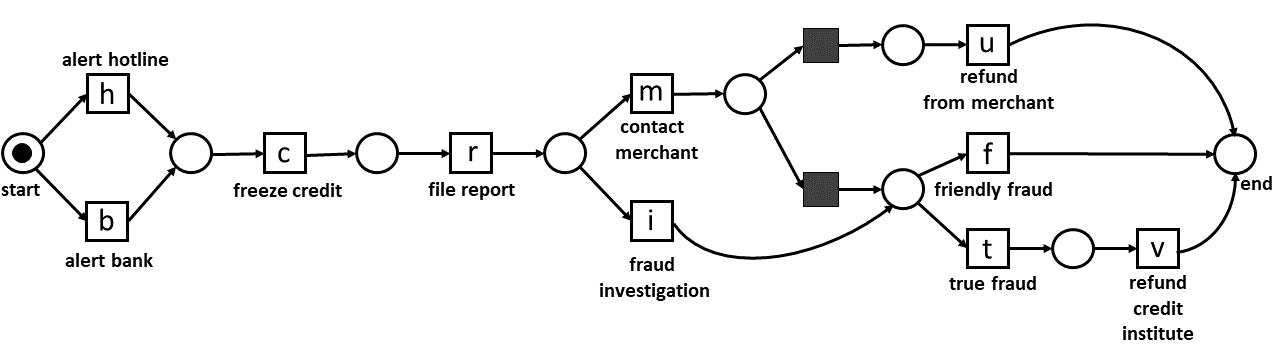
\includegraphics[width=1\columnwidth]{figures/petrinet_cc.png}
	\caption{A Petri net visualizing the remote credit card fraud investigation process. This model allows for 10 possible activity traces.}
	\label{fig: petrinet}
	%width=1\columnwidth
\end{figure}

Note that for simplicity, we have used single letters to represent the activity labels in the Petri net transitions.
Some possible traces in this process are for example:
$\langle h,c,r,m,u \rangle$,
$\langle b,c,r,m,f \rangle$,
$\langle h,c,r,i,f \rangle$ and
$\langle b,c,r,i,t,v \rangle$.

Suppose that the credit card company wants to do conformance checking to identify deviant process runs.
While some non-conforming cases may indicate that an investigation was not carried out transparently, other frequently reoccurring deviations may indicate that the process model should be updated as it does not reflect the real process anymore.
The company uses conformance checking to become aware of both these aspects.

In the following, we analyze a process instance identifying cardholder with ID 5167 and containing 6 events, some of which are uncertain (shown in Table \ref{table: credit card case}).
%
%
%
\begin{table}[h]
\caption{Example of an uncertain case from the credit card fraud investigation process.}
	%\centering
	%\hspace{-1cm}
	%\scriptsize
	\begin{adjustbox}{width=\columnwidth,center}
	\begin{tabular}{ccccc}
		\textbf{Case ID} & \textbf{Event ID} & \textbf{Activity} & \textbf{Timestamp} & \textbf{Type}\\ \hline
	%\multicolumn{1}{c}{\cellcolor{black!30}\textbf{Case ID}} & 
  %\multicolumn{1}{c}{\cellcolor{black!30}\textbf{Event ID}} &
  %\multicolumn{1}{c}{\cellcolor{black!30}\textbf{Timestamp}}
  %\\\hline
	\multicolumn{1}{|c|}{5167} & 
	\multicolumn{1}{|c|}{$e_1$} &
	\multicolumn{1}{|c|}{$h$ (alert hotline)} &
  	\multicolumn{1}{c|}{\begin{tabular}[c]{@{}c@{}} 05-10-2020 23:00
  	\end{tabular}}&
	\multicolumn{1}{|c|}{$!$} 
\\ \hline
	\multicolumn{1}{|c|}{5167} & 
	\multicolumn{1}{|c|}{$e_2$} &
	\multicolumn{1}{|c|}{$c$ (freeze credit)} &
  	\multicolumn{1}{c|}{\begin{tabular}[c]{@{}c@{}} 06-10-2020 \end{tabular}}&
	\multicolumn{1}{|c|}{$!$} 
\\ \hline
	\multicolumn{1}{|c|}{5167} & 
	\multicolumn{1}{|c|}{$e_3$} &
	\multicolumn{1}{|c|}{$r$ (file report)} &
  	\multicolumn{1}{c|}{\begin{tabular}[c]{@{}c@{}} $U$(05-10-2020 20:00, 06-10-2020 10:00) \end{tabular}}&
	\multicolumn{1}{|c|}{$!$} 
\\ \hline
	\multicolumn{1}{|c|}{5167} & 
	\multicolumn{1}{|c|}{$e_4$} &
	\multicolumn{1}{|c|}{$i$ (fraud investigation)} &
  	\multicolumn{1}{c|}{\begin{tabular}[c]{@{}c@{}} 09-10-2020 10:00 \end{tabular}}&
	\multicolumn{1}{|c|}{$!$} 
\\ \hline
	\multicolumn{1}{|c|}{5167} & 
	\multicolumn{1}{|c|}{$e_5$} &
	\multicolumn{1}{|c|}{\shortstack{$\{f: 0.3$ (friendly fraud), \\ $t: 0.7$ (true fraud)$\}$}} &
  	\multicolumn{1}{c|}{\begin{tabular}[c]{@{}c@{}} 14-10-2020 09:00 \end{tabular}}&
	\multicolumn{1}{|c|}{$!$} 
\\ \hline
	\multicolumn{1}{|c|}{5167} & 
	\multicolumn{1}{|c|}{$e_6$} &
	\multicolumn{1}{|c|}{$v$ (refund credit institute)} &
  	\multicolumn{1}{c|}{\begin{tabular}[c]{@{}c@{}} 15-10-2020 10:00 \end{tabular}}&
	\multicolumn{1}{|c|}{$?$} 
\\ \hline
	\end{tabular}
	\label{table: credit card case}
	\end{adjustbox}
\end{table} 
%
%
%
Suppose that in the first half of October 2020, the company was implementing a new system for automatic event data generation.
During this time, the event data regarding the credit card fraud investigation process often had to be inserted manually from the employees.
Such manual recordings were subject to inaccuracies, leading to imprecise or missing data affecting the cases during this period.
The process instance from Table \ref{table: credit card case} is one of the affected instances.
Here, events $e_2,e_3,e_5,e_6$ are uncertain.
The timestamp of event $e_2$ is not precise enough, so the possible timestamp lies between 06-10-2020 00:00 and 07-10-2020 00:00.
Event $e_3$ has happened some time between 20:00 on October 5th and 10:00 on October 6th. 
Event $e_5$ has two possible activity labels: $f$ with probability $0.3$ and $t$ with probability $0.7$.
Refunding the customer (event $e_6$) has been recorded in the system but the customer has not received the money yet, that is why the event is indeterminate.
%
%
%
%
\begin{figure}[h] 
\centering

	\begin{tikzpicture}[->,>=stealth',shorten >=1pt,node 						distance=2.5cm,auto,main node/.style={circle,draw,align=center}]
	%\draw [help lines] (0,0) grid (7,2);
	\node[main node,label=above:  {$h$}] (A) at (0,2) {$e_1$};
	\node[main node,label=above: {$c$}] (B) at (2,2) {$e_2$};
	\node[main node,label=above:  {$r$}] (C) at (1,0) {$e_3$};
	\node[main node,label=above:  {$i$}] (D) at (4,1) {$e_4$};
	\node[main node,label=above: {$\{f,t\}$}] (E) at (6,1) {$e_5$};
	\node[main node,dashed,label=above: {$v$}] (F) at (8,1) {$e_6$};
	
	\path
	(A) edge (B)
	(B) edge (D)
	(C) edge (D)
	(D) edge (E)
	(E) edge (F)
	

	;
	\end{tikzpicture}
	\caption{The behavior graph of event set from Table \ref{table: credit card case}. The labels above the nodes indicate the activities executed by each event, the dashed nodes indicate indeterminate events while the graph structure incorporates the uncertainty in timestamps.
	}
	\label{fig: beh graph credit card}
\end{figure}
%
%
%

Fig. \ref{fig: beh graph credit card} shows the behavior graph of this event set.
After computing the valid permutations on set $E=\{e_1,...,e_6\}$, we obtain 
$\mathcal{R}_e$=$\{
\underbrace{\langle e_1,e_2,e_3,e_4,e_5,e_6\rangle}_{s_e^1}$, 
$\underbrace{\langle e_1,e_3,e_2,e_4,e_5,e_6\rangle}_{s_e^2}$,
$\underbrace{\langle e_3,e_1,e_2,e_4,e_5,e_6\rangle}_{s_e^3}$,
$\underbrace{\langle e_1,e_2,e_3,e_4,e_5\rangle}_{s_e^4}$,
$\underbrace{\langle e_1,e_3,e_2,e_4,e_5\rangle}_{s_e^5}$,
$\underbrace{\langle e_3,e_1,e_2,e_4,e_5\rangle}_{s_e^6}
\}$.
Each of these sequences enables two activity traces:
\begin{align*}
A(s_e^1)&= \{ \underbrace{\langle h,c,r,i,f,v \rangle}_{s_a^{1'}}, \underbrace{\langle h,c,r,i,t,v \rangle}_{s_a^{1''}}\} ~,~~
A(s_e^2)= \{ \underbrace{\langle h,r,c,i,f,v \rangle}_{s_a^{2'}}, \underbrace{\langle h,r,c,i,t,v \rangle}_{s_a^{2''}}\}, \\
A(s_e^3)&= \{ \underbrace{\langle r,h,c,i,f,v \rangle}_{s_a^{3'}}, \underbrace{\langle r,h,c,i,t,v \rangle}_{s_a^{3''}}\} ~,~~
A(s_e^4)= \{ \underbrace{\langle h,c,r,i,f \rangle}_{s_a^{4'}}, \underbrace{\langle h,c,r,i,t \rangle}_{s_a^{4''}}\}, \\
A(s_e^5)&= \{ \underbrace{\langle h,r,c,i,f \rangle}_{s_a^{5'}}, \underbrace{\langle h,r,c,i,t \rangle}_{s_a^{5''}}\} ~,~~
A(s_e^6)= \{ \underbrace{\langle r,h,c,i,f \rangle}_{s_a^{6'}}, \underbrace{\langle r,h,c,i,t \rangle}_{s_a^{6''}}\}.
\end{align*}
Note that each activity trace is only enabled by a single event trace.
This is always the case when there are no two events sharing a common activity label.

Each event sequence enables two activity sequences because event $e_5$ has two possible activity labels.
Since for events $e \in E \setminus \{e_5\}$, we have $f_A^e$ equal to 1 for their corresponding unique activity label, the probability that an event sequence $s_e \in \mathcal{R}_e$ has some activity trace $s_a \in A(s_e)$ only depends on whether the trace $s_a$ contains activity $f$ or $t$.
Thus, for traces $s_a^{1'},s_a^{2'},s_a^{3'},s_a^{4'},s_a^{5'},s_a^{6'}$ and their unique enabling sequences, we always have \mbox{$P_a(s_a^{i'} \mid s_e^{i})$} $= f_A^{e_5}(f) = 0.3$, where $i \in \{1,...,6\}$.
Similarly, for traces $s_a^{1''},s_a^{2''},s_a^{3''},s_a^{4''},s_a^{5''},s_a^{6''}$ and their unique enabling sequences, we always have \mbox{$P_a(s_a^{i''} \mid s_e^{i})$} $= f_A^{e_5}(t) = 0.7$, where \mbox{$i \in \{1,...,6\}$}.

Next, we calculate the $P_e$ values for the 6 possible event sequences in $\mathcal{R}_e$.
First, we determine that the uncertain process instance has weak uncertainty in timestamps and strong uncertainty in the event qualifier, so it belongs to the $[T]_{\mathbb{W}}[O]_{\mathbb{S}}$ scenario.
Since there is only one indeterminate event, we have $k = 2$.
The $P_e$-values are displayed in Table \ref{table: Pe values}.

%
%
%
\begin{table}[h]
\caption{The possible event sequences of the process instance from Table \ref{table: credit card case} and their probabilities.}
	\centering
	\begin{tabular}{ccc}
		\textbf{Event sequences} & \textbf{$I(s_e)$} & \textbf{$P_e(s_e)$}
		\\ \hline
	%\multicolumn{1}{c}{\cellcolor{black!30}\textbf{Case ID}} & 
  %\multicolumn{1}{c}{\cellcolor{black!30}\textbf{Event ID}} &
  %\multicolumn{1}{c}{\cellcolor{black!30}\textbf{Timestamp}}
  %\\\hline
	\multicolumn{1}{|c|}{$~ s_e^1:~\langle e_1,e_2,e_3,e_4,e_5,e_6\rangle ~$} & 
	\multicolumn{1}{|c|}{$~ 0.14859 ~$} &
	\multicolumn{1}{|c|}{$~ 0.07429 ~$} 
\\ \hline
	\multicolumn{1}{|c|}{$s_e^2:~\langle e_1,e_3,e_2,e_4,e_5,e_6\rangle$} & 
	\multicolumn{1}{|c|}{$0.77989$} &
	\multicolumn{1}{|c|}{$0.38995$} 
\\ \hline
	\multicolumn{1}{|c|}{$s_e^3:~\langle e_3,e_1,e_2,e_4,e_5,e_6\rangle$} & 
	\multicolumn{1}{|c|}{$0.07151$} &
	\multicolumn{1}{|c|}{$0.03576$} 
\\ \hline
	\multicolumn{1}{|c|}{$s_e^4:~\langle e_1,e_2,e_3,e_4,e_5\rangle$} & 
	\multicolumn{1}{|c|}{$0.14859$} &
	\multicolumn{1}{|c|}{$0.07429$} 
\\ \hline
	\multicolumn{1}{|c|}{$s_e^5:~\langle e_1,e_3,e_2,e_4,e_5\rangle$} & 
	\multicolumn{1}{|c|}{$0.77989$} &
	\multicolumn{1}{|c|}{$0.38995$} 
\\ \hline
	\multicolumn{1}{|c|}{$s_e^6:~\langle e_3,e_1,e_2,e_4,e_5\rangle$} & 
	\multicolumn{1}{|c|}{$0.07151$} &
	\multicolumn{1}{|c|}{$0.03576$} 
\\ \hline
	\end{tabular}
	\label{table: Pe values}
\end{table} 
%
%
%
One can notice that the $I$ values only depend on the ordering of the first three events, which are also the only ones with overlapping timestamps.
Since the indeterminate event $e_6$ does not overlap with any other event, pairs of sequences where the first three events have the same order also have the same probability.
This reflects our assumption that the occurrence and non-occurrence of $e_6$ are both equally possible.
Table \ref{table: p values} displays the calculations for the computation of the $\textbf{p}$ values for all activity traces.
Note that the numbers in both Tables \ref{table: Pe values} and \ref{table: p values} have been rounded.

%
%
%
\begin{table}[h]
	\caption{The set of possible activity traces of the example from Table \ref{table: credit card case}, their enablers, their probabilities and their conformance scores. The conformance score is equal to the cost of the optimal alignment between the trace and the Petri net in Fig. \ref{fig: petrinet}. In this example, every activity trace has only one event sequence enabling it.}
	\centering
	\begin{tabular}{cccc}
		\textbf{Activity trace $s_a$} & \textbf{Enablers}($s_a$) & \textbf{$\textbf{p}(s_a)$} & \textbf{$conf(s_a,M)$}
		\\ \hline
	%\multicolumn{1}{c}{\cellcolor{black!30}\textbf{Case ID}} & 
  %\multicolumn{1}{c}{\cellcolor{black!30}\textbf{Event ID}} &
  %\multicolumn{1}{c}{\cellcolor{black!30}\textbf{Timestamp}}
  %\\\hline
	\multicolumn{1}{|c|}{$~s_a^{1'}: ~ \langle h,c,r,i,f,v \rangle~$} & 
	\multicolumn{1}{|c|}{$~ s_e^1 ~$} & 
	\multicolumn{1}{|c|}{$~ P_e(s_e^1) \cdot P_a(s_a^{1'} \mid s_e^1) = 0.02229 ~$} &
	\multicolumn{1}{|c|}{$~ 1 ~$}
\\ \hline
	\multicolumn{1}{|c|}{$s_a^{1''}: ~ \langle h,c,r,i,t,v \rangle$} & 
	\multicolumn{1}{|c|}{$s_e^1$} & 
	\multicolumn{1}{|c|}{$~ P_e(s_e^1) \cdot P_a(s_a^{1''} \mid s_e^1) = 0.05201 ~$} &
	\multicolumn{1}{|c|}{$~ 0 ~$}
\\ \hline
	\multicolumn{1}{|c|}{$s_a^{2'}: ~ \langle h,r,c,i,f,v\rangle$} & 
	\multicolumn{1}{|c|}{$s_e^2$} & 
	\multicolumn{1}{|c|}{$~ P_e(s_e^2) \cdot P_a(s_a^{2'} \mid s_e^2) =  0.11698~$} &
	\multicolumn{1}{|c|}{$~ 3 ~$}
\\ \hline
	\multicolumn{1}{|c|}{$s_a^{2''}: ~ \langle h,r,c,i,t,v\rangle$} & 
	\multicolumn{1}{|c|}{$s_e^2$} & 
	\multicolumn{1}{|c|}{$~ P_e(s_e^2) \cdot P_a(s_a^{2''} \mid s_e^2) = 0.27296~$} &
	\multicolumn{1}{|c|}{$~ 2 ~$}
\\ \hline
	\multicolumn{1}{|c|}{$s_a^{3'}: ~ \langle r,h,c,i,f,v\rangle$} & 
	\multicolumn{1}{|c|}{$s_e^3$} & 
	\multicolumn{1}{|c|}{$~ P_e(s_e^3) \cdot P_a(s_a^{3'} \mid s_e^3) = 0.01073~$} &
	\multicolumn{1}{|c|}{$~ 3 ~$}
\\ \hline
	\multicolumn{1}{|c|}{$s_a^{3''}: ~ \langle r,h,c,i,t,v\rangle$} & 
	\multicolumn{1}{|c|}{$s_e^3$} & 
	\multicolumn{1}{|c|}{$~ P_e(s_e^3) \cdot P_a(s_a^{3''} \mid s_e^3) = 0.02503~$} &
	\multicolumn{1}{|c|}{$~ 2 ~$}
\\ \hline
\multicolumn{1}{|c|}{$~s_a^{4'}: ~ \langle h,c,r,i,f \rangle~$} & 
	\multicolumn{1}{|c|}{$~ s_e^4 ~$} & 
	\multicolumn{1}{|c|}{$~ P_e(s_e^4) \cdot P_a(s_a^{4'} \mid s_e^4) = 0.02229 ~$} &
	\multicolumn{1}{|c|}{$~ 0 ~$}
\\ \hline
	\multicolumn{1}{|c|}{$s_a^{4''}: ~ \langle h,c,r,i,t \rangle$} & 
	\multicolumn{1}{|c|}{$s_e^4$} & 
	\multicolumn{1}{|c|}{$~ P_e(s_e^4) \cdot P_a(s_a^{4''} \mid s_e^4) = 0.05201~$} &
	\multicolumn{1}{|c|}{$~ 1 ~$}
\\ \hline
	\multicolumn{1}{|c|}{$s_a^{5'}: ~ \langle h,r,c,i,f\rangle$} & 
	\multicolumn{1}{|c|}{$s_e^5$} & 
	\multicolumn{1}{|c|}{$~ P_e(s_e^5) \cdot P_a(s_a^{5'} \mid s_e^5) = 0.11698~$} &
	\multicolumn{1}{|c|}{$~ 2 ~$}
\\ \hline
	\multicolumn{1}{|c|}{$s_a^{5''}: ~ \langle h,r,c,i,t\rangle$} & 
	\multicolumn{1}{|c|}{$s_e^5$} & 
	\multicolumn{1}{|c|}{$~ P_e(s_e^5) \cdot P_a(s_a^{5''} \mid s_e^5) = 0.27296~$} &
	\multicolumn{1}{|c|}{$~ 3 ~$}
\\ \hline
	\multicolumn{1}{|c|}{$s_a^{6'}: ~ \langle r,h,c,i,f\rangle$} & 
	\multicolumn{1}{|c|}{$s_e^6$} & 
	\multicolumn{1}{|c|}{$~ P_e(s_e^6) \cdot P_a(s_a^{6'} \mid s_e^6) = 0.01073~$} &
	\multicolumn{1}{|c|}{$~ 2 ~$}
\\ \hline
	\multicolumn{1}{|c|}{$s_a^{6''}: ~ \langle r,h,c,i,t\rangle$} & 
	\multicolumn{1}{|c|}{$s_e^6$} & 
	\multicolumn{1}{|c|}{$~ P_e(s_e^6) \cdot P_a(s_a^{6''} \mid s_e^6) = 0.02503~$} &
	\multicolumn{1}{|c|}{$~ 3 ~$}
\\ \hline
	\end{tabular}
	\label{table: p values}
\end{table} 
% 
%
%
Now we can compute the expected conformance score for the uncertain process instance with event set $E=\{e_1,...,e_6\}$:
\begin{align*}
\overline{Conf}(E) &= \sum_{s_a \in \mathcal{R}_a(E)} \textbf{p}(s_a) \cdot conf(s_a,M) \\
&= 0.02229 \cdot 1 + 0.05201 \cdot 0 + 0.11698 \cdot 3 + 0.27296 \cdot 2 \\ 
&+ 0.01073 \cdot 3 + 0.02503 \cdot 2 +
0.02229 \cdot 0 + 0.05201 \cdot 1 \\
&+ 0.11698 \cdot 2 + 0.27296 \cdot 3 + 0.01073 \cdot 2 + 0.02503 \cdot 3 \\
&= 2.2028.
\end{align*}

Given that the information on uncertainty and the assumptions made regarding the independencies within that information are correct, this conformance score is a better estimate of the real conformance score compared to taking the best, worst or average scores with values 0, 3 and 1.75 respectively. 
%Assuming uniform distribution over the above set of activity trace realizations, the weighted conformance score would equate the average conformance score of 1.75.\\


\section{Validation of Probability Estimates}
In this section, we compute the probability estimates for the trace realizations of some example process instance, and then validate those estimates on two different aspects:
First, we show how the expected conformance score of an uncertain trace might be much different than taking the best, worst or average score.
Second, we show that the obtained estimate values are correct by conducting a Monte Carlo simulation on the behavior net of the uncertain trace.
We run the simulation 100000 times and then compare the frequency of each trace realization during the simulation with the probability estimate we computed with our method.
The experiment has been implemented in Python\footnote{\url{https://github.com/biankabakullari/UncertainLogProbabilities/tree/master/code/Probabilities_Validation}}.
%
%
%
%
\begin{figure}[h] 
\centering

	\begin{tikzpicture}[->,>=stealth',shorten >=1pt,node 						distance=2.5cm,auto,main node/.style={circle,draw,align=center}]
	%\draw [help lines] (0,0) grid (8,5);
	\node[main node,label=above:  \large{$a$}] (A) at (2,2) {$e_1$};
	\node[main node,label=above: \Large{$\substack{b:~0.9\\ c:~0.1}$}] (B) at (4,3) {$e_2$};
	\node[main node,dashed,label=above: \large{$d$}, label=below:  \Large{$\substack{!:~0.2\\ ?:~0.8}$}] (C) at (4,1) {$e_3$};
	\node[main node,label=above:  \large{$e$}] (D) at (6,2) {$e_4$};

	
	\path
	(A) edge (B)
	(A) edge (C)
	(C) edge (D)
	(B) edge (D)
	

	;
	\end{tikzpicture}
	\caption{The behavior graph of a process instance with strong uncertainty in timestamps and weak uncertainty in activities and event type.
	}
	\label{fig: validation beh graph}
\end{figure}
%
%
%
%
%
%
\begin{table}[h]
	\begin{adjustbox}{width=\columnwidth,center}
	\begin{tabular}{cccc}
		\textbf{Trace $s_a$} & \textbf{Enablers}($s_a$) & \textbf{$\textbf{p}(s_a)$} & \textbf{$conf(s_a,M)$}
		\\ \hline
	%\multicolumn{1}{c}{\cellcolor{black!30}\textbf{Case ID}} & 
  %\multicolumn{1}{c}{\cellcolor{black!30}\textbf{Event ID}} &
  %\multicolumn{1}{c}{\cellcolor{black!30}\textbf{Timestamp}}
  %\\\hline
	\multicolumn{1}{|c|}{$~s_a^{1}: ~ \langle a,b,e \rangle~$} &                                                 	\multicolumn{1}{|c|}{$~s_e^{1}: ~ \langle e_1,e_2,e_4 \rangle~$} & 
	\multicolumn{1}{|c|}{$P_e(s_e^1) \cdot P_a(s_a^1 | s_e^1) 
		=  0.8 \cdot 0.9  = 0.72$}  & 
	\multicolumn{1}{|c|}{$3$} 
\\ \hline  
	\multicolumn{1}{|c|}{$s_a^{2}: ~ \langle a,b,d,e \rangle$} & 
	\multicolumn{1}{|c|}{$s_e^2: \langle e_1,e_2,e_3,e_4 \rangle$} & 
	\multicolumn{1}{|c|}{$~ P_e(s_e^2) \cdot P_a(s_a^2 \mid s_e^2) = (0.5 \cdot 0.2) \cdot 0.9 = 0.09 ~$} &
	\multicolumn{1}{|c|}{$~ 2 ~$}
\\ \hline
	\multicolumn{1}{|c|}{$s_a^{3}: ~ \langle a,d,b,e \rangle$} & 
	\multicolumn{1}{|c|}{$s_e^3: \langle e_1,e_3,e_2,e_4 \rangle$} & 
	\multicolumn{1}{|c|}{$~ P_e(s_e^3) \cdot P_a(s_a^3 \mid s_e^3) =  (0.5 \cdot 0.2) \cdot 0.9 = 0.09 ~$} &
	\multicolumn{1}{|c|}{$~ 2 ~$}
\\ \hline
	\multicolumn{1}{|c|}{$~s_a^{4}: ~ \langle a,c,e \rangle~$} &                                                       	\multicolumn{1}{|c|}{$~s_e^{4}: ~ \langle e_1,e_2,e_4 \rangle~$} & 
	\multicolumn{1}{|c|}{$P_e(s_e^4) \cdot P_a(s_a^4 | s_e^4)
		=0.8 \cdot 0.1 = 0.08$ }  & 
	\multicolumn{1}{|c|}{$1$}  
\\ \hline  
	\multicolumn{1}{|c|}{$s_a^{5}: ~ \langle a,c,d,e \rangle$} & 
	\multicolumn{1}{|c|}{$s_e^5: \langle e_1,e_2,e_3,e_4 \rangle$} & 
	\multicolumn{1}{|c|}{$~ P_e(s_e^5) \cdot P_a(s_a^5 \mid s_e^5) = (0.5 \cdot 0.2) \cdot 0.1 = 0.01~$} &
	\multicolumn{1}{|c|}{$~ 0 ~$}
\\ \hline
	\multicolumn{1}{|c|}{$s_a^{6}: ~ \langle a,d,c,e \rangle$} & 
	\multicolumn{1}{|c|}{$s_e^6: \langle e_1,e_3,e_2,e_4 \rangle$} & 
	\multicolumn{1}{|c|}{$~ P_e(s_e^6) \cdot P_a(s_a^6 \mid s_e^6) = (0.5 \cdot 0.2) \cdot 0.1 = 0.01~$} &
	\multicolumn{1}{|c|}{$~ 0 ~$}
\\ \hline
	\end{tabular}
	\end{adjustbox}
	\caption{The set of activity trace realizations of the process instance from Fig. \ref{fig: validation beh graph}, their enablers, their probabilities and their conformance scores. The conformance score is equal to the cost of the optimal alignment between the trace and the Petri net in Fig. \ref{fig: validation model}.}
	\label{table: validation estimates}
\end{table} 
% 
%
%
%

The process instance of our example has strong uncertainty in timestamps and weak uncertainty in activities and event type.
It consists of 4 events: $e_1,e_2,e_3$ and $e_4$, where $e_2$ and $e_3$ have overlapping timestamps.
Event $e_2$ executes $b$ with probability 0.9 and $c$ with probability 0.1.
Event $e_3$ is indeterminate and there is a probability of 0.2 that it did not occurr.
Fig. \ref{fig: validation beh graph} shows the corresponding behavior graph.
The first two columns from Table \ref{table: validation estimates} list all the possible activity traces beside the event sequences enabling them.
The third column shows how the probabilities are obtained for each trace realization considering the $[T]_{\mathbb{S}}[A,O]_{\mathbb{W}}$ uncertainty scenario.
In the last column, the alignment scores between each possible trace and the model from Fig. \ref{fig: validation model} are shown.
Notice how in this specific example, traces that show a worse conformance score are the most likely ones, while the conforming traces are very unlikely in comparison.
The uncertain trace in the example has an expected conformance score of 2.6.
Assuming uniform distribution over the trace realizations would yield a more optimistic expected conformance score of approximately 1.33.
Moreover, considering the uncertain trace as conforming because one trace realization has conformance cost equal to 0 would be even further from our computed score.

%
%
%
\begin{figure}
	\centering
	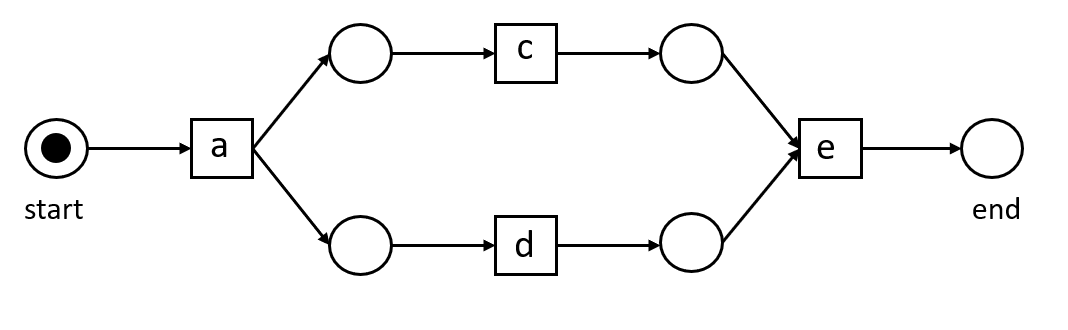
\includegraphics[width=0.8\columnwidth]{figures/model_validation.png}
	\caption{A Petri net visualizing the normative model of the process during which the instance from Table \ref{table: validation estimates} was executed.}
	\label{fig: validation model}
	%width=1\columnwidth
\end{figure}
%
%
%
%
%
%
\begin{figure}
	\centering
	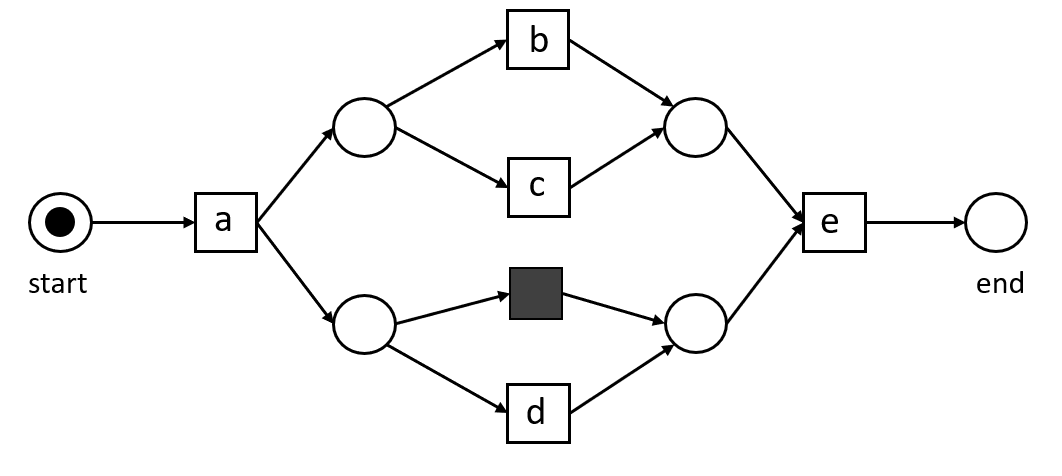
\includegraphics[width=0.8\columnwidth]{figures/behaviornet.png}
	\caption{The behavior net obtained from the behavior graph in Fig. \ref{fig: validation beh graph}.
	The weights of the transitions are chosen so that they simulate weak uncertainty in activities and event type, and strong uncertainty in timestamps.}
	\label{fig: behavior net}
	%width=1\columnwidth
\end{figure}
%
%
%
%
%
%

For the same process instance from Fig. \ref{fig: validation beh graph}, we now validate our obtained probability estimates quantitatively by means of the Monte Carlo simulation approach.
First, we construct the behavior net corresponding to the uncertain process instance which is shown in Fig. \ref{fig: behavior net}.
The set of replayable traces in this behavior net is exactly the set of activity trace realizations for the uncertain instance.
Then, we run a simulator on the behavior net 100000 times producing 100000 possible traces.
After each run, we divide the accumulated count of each trace variant by the number of runs, and compare those values to our probability estimates.
The simulator we use here is provided in the PM4Py library and it is called a stochastic simulator.
The stochastic simulator picks in every step of the simulation one transition out of the set of enabled transitions according to a stochastic map, assigning a weight to each transition in the Petri net (here: behavior net). 
The next transition to fire is picked randomly following a probability distribution over the set of enabled transitions. 
If not specified otherwise, each transition $t$ initially has $weight(t)=1$ in the stochastic map. 
In each step, a new probability distribution is computed over the set of enabled transitions by dividing their weight with the sum of the weights of the enabled transitions (normalization). 
By default, this distribution is always uniform. 
One can also assign specific weights to the transitions. 
These weights become relevant by (potentially) leading to non-uniform distributions when the simulator randomly picks the next transition to fire. 
There are two scenarios for when the weights affect the random choice the simulator: 
\begin{itemize}
\item The XOR-split:
The transitions in an XOR-split pairwise exclude each-other. 
How often each of them is chosen will roughly reflect how their weights compare to each-other.
\item The AND-split:
All paths following the AND-split will certainly be taken by the simulator. 
\end{itemize}
Since the weights in the Petri net are only defined for transitions and not explicitly for arcs, which path is taken first (or second and so on) depends on the probability distribution over all enabled transitions at that moment. 
The probability of one particular path being taken (meaning one of its transitions is fired) is then equal to the sum of the weights of the transitions that are enabled following that particular path over the sum of the weights of all enabled transitions over all paths in the AND-split.
To simulate uncertainty in activities, events and timestamps we do the following: 
Possible activities executed by the same event appearing in an XOR-split in the behavior net get weights so that in relation to each-other their weights reflect how much more likely one activity is compared to the other one(s). 
Whether an event with a unique activity is executed or not (uncertainty in event type), is equivalently modeled as an XOR-choice between a visible transition and a silent one in the behavior net (see Def. \ref{def: bn}). 
If there are two or more possible acitivities for an indeterminate event, then the sum of the weights of the visible transitions in relation to the weight of the silent transition should be the same as in the distribution given in the event type uncertainty information.
Regarding timestamps, through the simulator we can only simulate strong uncertainty, that is, uniform distribution over the possible event orderings. 
Whenever there are events with overlapping timestamps, these appear in an AND-split in the behavior net. 
Which path of the AND-split is taken first (out of the ones that are enabled) signals which event is executed at that moment.
Since one event might have many possible activities and thus transitions, to simulate a uniform distrubution over the choice of the path at any moment, the sum of transitions' weights enabled immediately after following each path should sum to 1.

In the following we formalize how one can determine the weights of the transitions in the behavior net, given a set of uncertain events that has the following properties:
\begin{itemize}
\item (*) There is either no uncertainty or there is strong uncertainty in timestamps.
\item (**) Each connected component of the corresponding interval graph is a clique.
\end{itemize}

The first property reflects the fact that by running a simulator on a behavior net, we can only simulate strong uncertainty in timestamps .
%Events sets satisfying the second property make it easier to generalize how the weights should be distributed over the set of enabled transitions following an AND-split.
If an uncertain event set $E$ satisfies the second property, from Proposition \ref{prop: clique} it follows that $E$ can be partitioned into $E=\langle E_1,...,E_m \rangle$, where $m = |CC(\mathcal{I}(E))|$ is the number of connected components of the interval graph, and for all $1 \leq i \leq m$ it holds that $\forall e,e' \in E_i: ~ e$ and $e'$ have overlapping timestamps.
Let $bn(E)$ be the behavior net of uncertain event set $E$ satisfying (*) and (**).
Let $(e,a) \in T$ be a visible transition related to some event $e \in E$ in the behavior net.
We assign a weight to $(e,a)$ the following way:
\begin{align*}
weight((e,a))  = \begin{cases}
	 \frac{1}{|\pi_a^{set}(e)|} & \mbox{if} \; \pi_o(e)=! \wedge \pi_a(e) \not \in F_{\mathcal{U}_A}, \\
	f_A^{e}(a) & \mbox{if} \; \pi_o(e)=! \wedge \pi_a(e)=f_A^e \in F_{\mathcal{U}_A},  \\
	\frac{1}{2} \cdot \frac{1}{|\pi_a^{set}(e)|} & \mbox{if} \; \pi_o(e) = ? \wedge \pi_a(e) \not \in F_{\mathcal{U}_A}, \\
	f_O^e(!) \cdot f_A^{e}(a) & \mbox{if} \; \pi_o(e)=f_O^e \in F_{\mathcal{U}_O} \wedge \pi_a(e)=f_A^e \in F_{\mathcal{U}_A}.
	\end{cases} 
\end{align*}

If $e \in E$ is an indeterminate event, then 
\begin{align*}
weight((e,\tau))  = \begin{cases}
	 \frac{1}{2} & \mbox{if} \; \pi_o(e)=?, \\
	f_O^{e}(?) & \mbox{if} \; \pi_o(e)=f_O^e \in  F_{\mathcal{U}_O}.
	\end{cases} 
\end{align*}

Note that according to the weight assignment function, if $e$ is determinate, then $\sum_{a \in \pi_a^{set}(e)} \allowbreak weight((e,a)) = 1$.
Otherwise, $\sum_{a \in \pi_a^{set}(e)} weight((e,a)) = f_O^{e}(!) = 1 - f_O^{e}(?) = 1 - weight((e,\tau))$.
By construction of the behavior net, for all $1 \leq i < j \leq m$, any transition related to an event in $E_j$ can only fire after all transitions corresponding to events from $E_i$ have fired.
Additionally, all transitions representing events from the same subset $E_i$ appear in an AND construct.
By definition of our weight function, whenever the transitions of some $e_i \in E_i$ are enabled (in an XOR construct), the probability of firing one of them is $1/k$, where $k$ is the number of events from $E_i$ for which none of the corresponding transitions have fired yet.
This way, there is always a uniform distribution over the set of enabled transitions representing overlapping events.

In our example behavior net, we assign weights $0.9$, $0.1$, $0.2$ and $0.8$ to transitions $b$, $c$, $d$ and $\tau$ (the silent transition) respectively.
In the beginning, only $a$ can fire.
Afterwards, $b$, $c$, $d$ or $\tau$ are picked, each being assigned probability $weight(\cdot)/ (0.9+0.1+0.8+0.2)$, yielding a probability distribution over the enabled transitions assigning weights $0.45,0.05,0.4,0.1$ to $b$, $c$, $d$ and $\tau$ respectively. 
Executing $b$ is still $0.9/0.1=0.45/0.05=9$ times more likely than executing $c$, and thus reflecting the weak uncertainty in activities, whereas executing $d$ is still $0.2/0.8=0.1/0.4=1/4$ times less likely than skipping it, and thus reflecting the weak uncertainty in the event type.
In the simulation, there is always the choice of whether the upper path is taken first ($b$ or $c$ fires first), or whether the lower path is taken (executing $d$ or skipping it). 
This decision is made when all four transitions: $b$, $c$, $d$ and $\tau$ make up the set of enabled transitions. 
For example, the probability of executing $b$ will be:
$weight(b)/(weight(b)+weight(c)+weight(d)+weight(\tau))$. 
Since taking the upper path first implies $e_2$ happening before $e_3$, whereas the lower path implies $e_3$ happening before $e_2$, and we have no information on which is more likely, we want each of those paths to be taken equally often. 
This happens whenever $weight(b) + weight(c)=weight(d)+weight(\tau)$, which holds by definition of our weight function.
By construction, whenever those three transitions are enabled, in roughly half the cases $b$ or $c$ will be executed first, and in the other half $d$ or $\tau$.
If $b$ or $c$ happens first, then executing $d$ in the next step will have probability 0.2/(0.8+0.2) = 0.2. 
If $d$ or $\tau$ fires first, then the enabled transitions will be $b$ and $c$, where $b$ will get probability 0.9 and $c$ probability 0.1.

Applying the stochastic simulator $n$ times on the the behavior net where the transitions have the particular weights we explained above, yields $n$ traces.
For each possible trace out of the 6 trace realizations for the uncertain process instance, dividing the frequency of that trace by $n$ yields a probability estimate for that trace.
As expected, Fig. \ref{fig: abe}-\ref{fig: adce} show how for greater $n$, this estimate converges to the probability estimate shown in Table \ref{table: validation estimates}, which was computed with our equations.
Though we run the simulator for 100000 rounds to obtain more reliable values, we also plot the results for $n$ going from 1 to 1000 runs, to show how the fluctuations of the probabilities decrease and converge to the expected value when $n$ increases.

\begin{figure}%
    \centering
    {{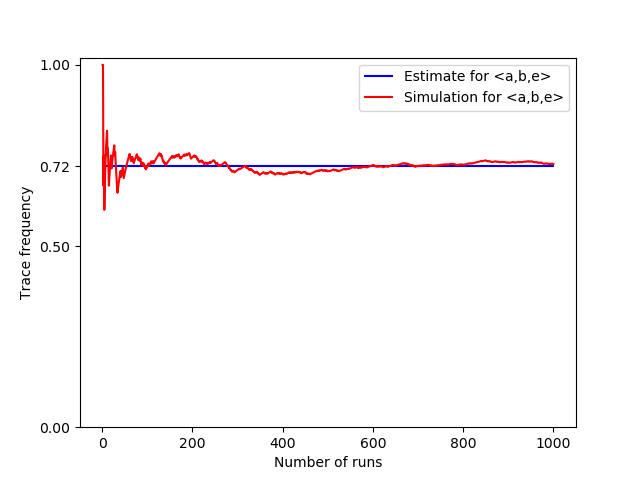
\includegraphics[width=12cm]{figures/abe1.png} }}%
    \qquad
   {{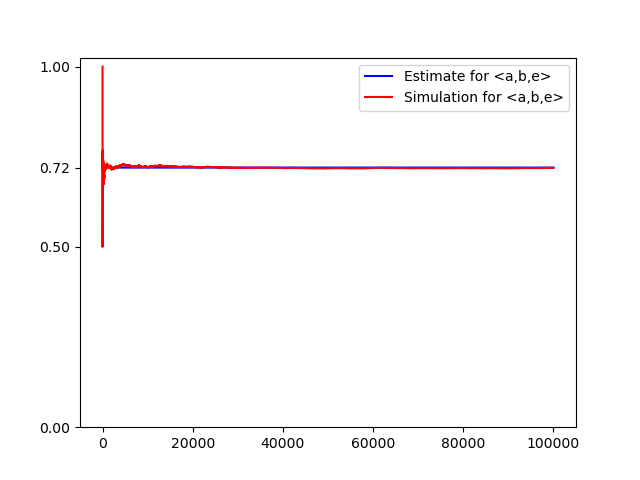
\includegraphics[width=12cm]{figures/abe100.png} }}%
    \caption{Two plots showing how the frequency of trace $\langle a,b,e \rangle$ converges to the expected value of $0.72$ over 1000 runs in the first plot, and 100000 runs in the second plot.}%
    \label{fig: abe}%
\end{figure}
%
%
%
%
%
%
%
\begin{figure}%
    \centering
    {{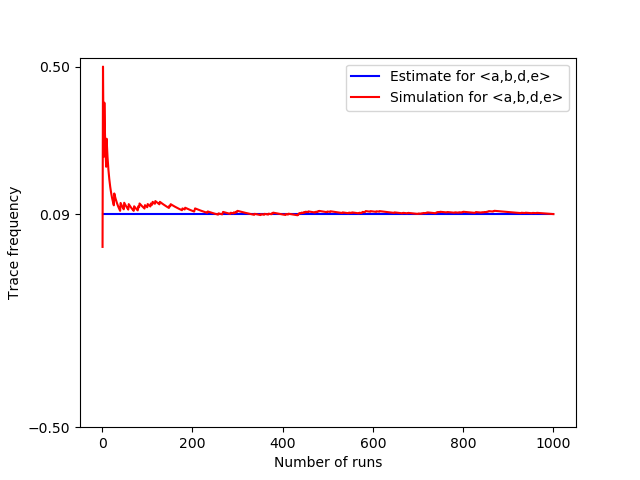
\includegraphics[width=12cm]{figures/abde1.png} }}%
    \qquad
    {{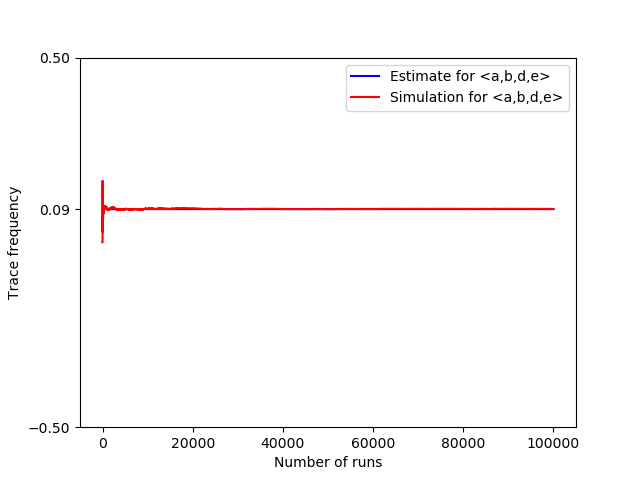
\includegraphics[width=12cm]{figures/abde100.png} }}%
    \caption{Two plots showing how the frequency of trace $\langle a,b,d,e \rangle$ converges to the expected value of $0.09$ over 1000 runs in the first plot, and 100000 runs in the second plot.}%
    \label{fig: abde}%
\end{figure}
%
%
%
%
%
%
\begin{figure}%
    \centering
    {{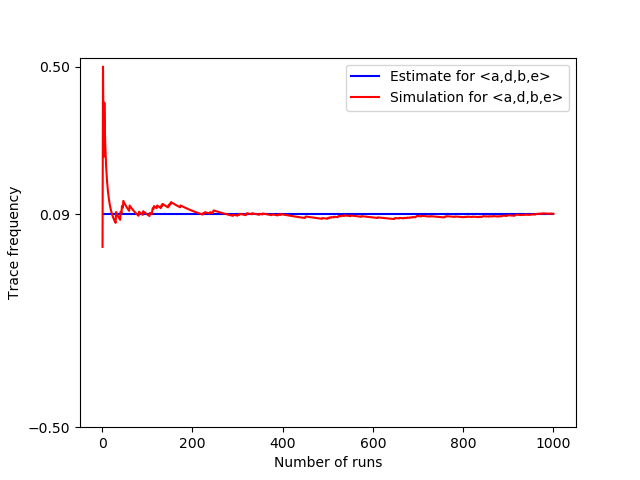
\includegraphics[width=12cm]{figures/adbe1.png} }}%
    \qquad
    {{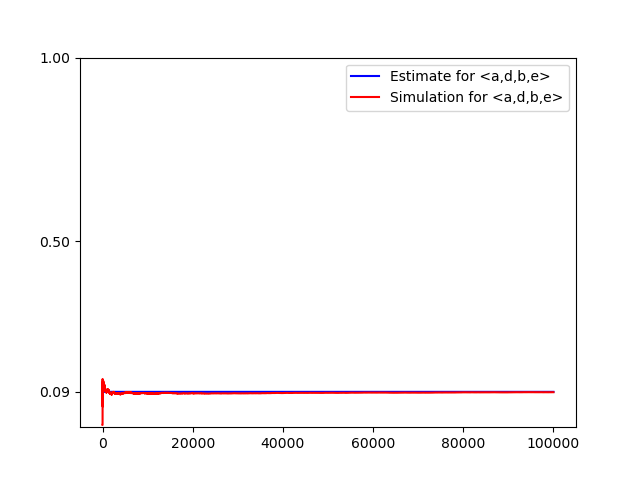
\includegraphics[width=12cm]{figures/adbe100.png} }}%
    \caption{Two plots showing how the frequency of trace $\langle a,d,b,e \rangle$ converges to the expected value of $0.09$ over 1000 runs in the first plot, and 100000 runs in the second plot.}%
    \label{fig: adbe}%
\end{figure}
%
%
%
%
%
%
\begin{figure}%
    \centering
    {{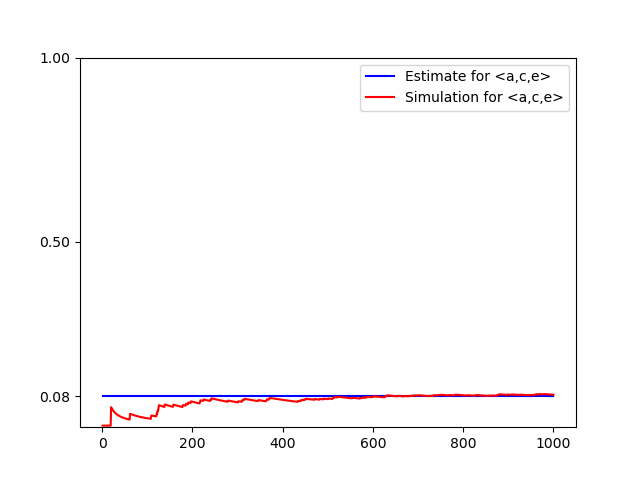
\includegraphics[width=12cm]{figures/ace1.png} }}%
    \qquad
    {{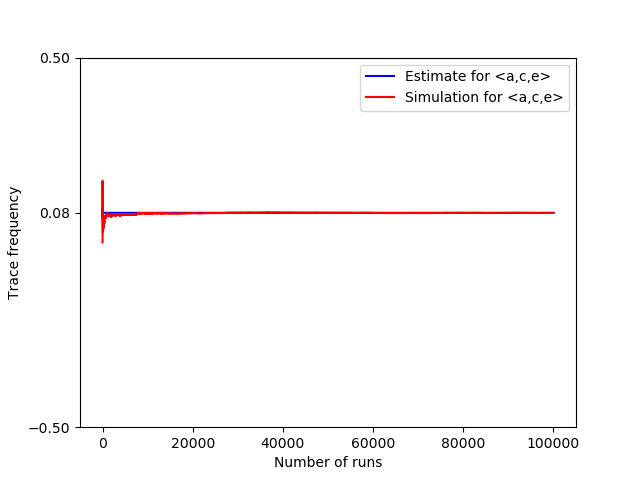
\includegraphics[width=12cm]{figures/ace100.png} }}%
    \caption{Two plots showing how the frequency of trace $\langle a,c,e \rangle$ converges to the expected value of $0.08$ over 1000 runs in the first plot, and 100000 runs in the second plot.}%
    \label{fig: ace}%
\end{figure}
%
%
%
%
%
%
\begin{figure}%
    \centering
    {{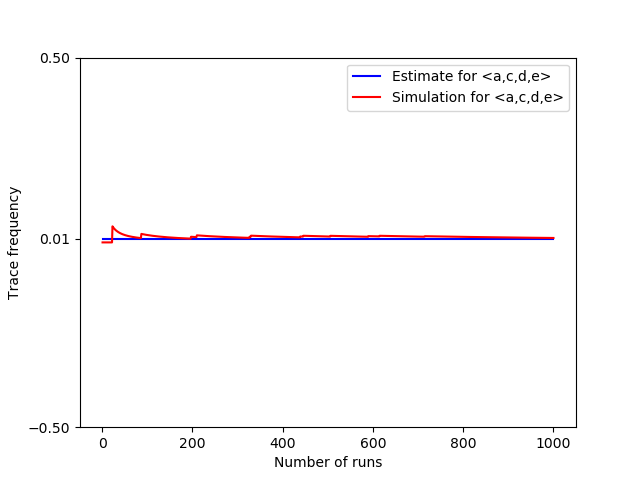
\includegraphics[width=12cm]{figures/acde1.png} }}%
    \qquad
    {{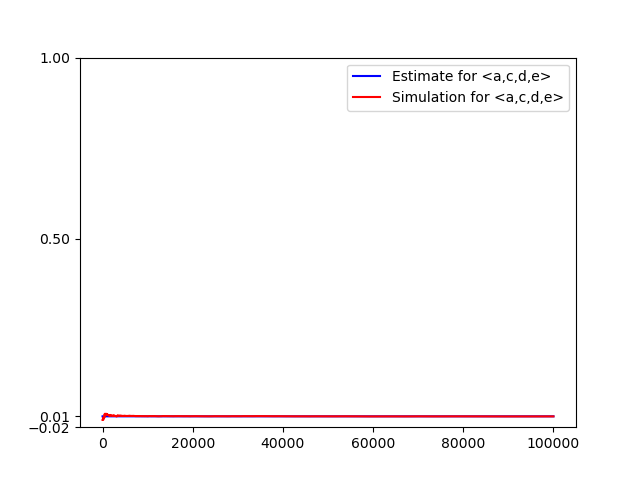
\includegraphics[width=12cm]{figures/acde100.png} }}%
    \caption{Two plots showing how the frequency of trace $\langle a,c,d,e \rangle$ converges to the expected value of $0.01$ over 1000 runs in the first plot, and 100000 runs in the second plot.}%
    \label{fig: acde}%
\end{figure}
%
%
%
%
%
%
\begin{figure}%
    \centering
    {{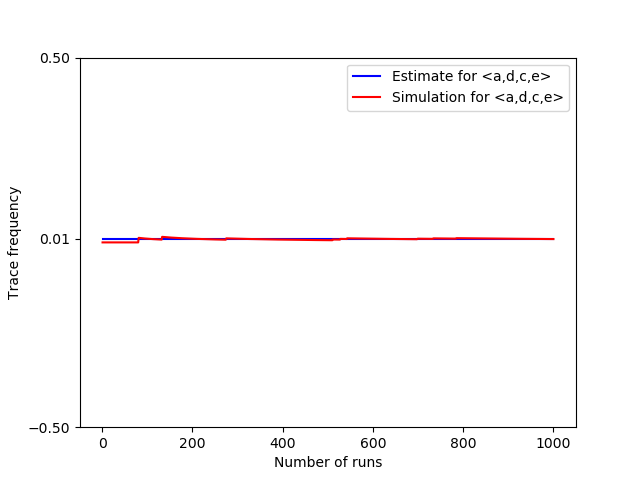
\includegraphics[width=12cm]{figures/adce1.png} }}%
    \qquad
    {{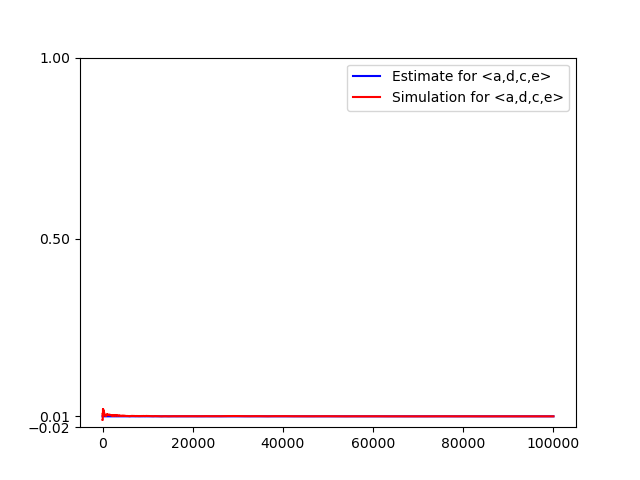
\includegraphics[width=12cm]{figures/adce100.png} }}%
    \caption{Two plots showing how the frequency of trace $\langle a,d,c,e \rangle$ converges to the expected value of $0.01$ over 1000 runs in the first plot, and 100000 runs in the second plot.}%
    \label{fig: adce}%
\end{figure}
%
%
%
%
%
%In the next section we try to improve our probability estimates and therefore the expected conformance score for each uncertain process instance.
%We assume that some trace realization is more likely if there are other traces in the log which are identical or similar to it.
To conclude, the Monte Carlo simulation showed that our estimated probabilities for the trace realizations match their relative frequencies when one simulates the behavior net of the corresponding uncertain process instance.

%
%
%
%
%
%
\newpage
\section{Estimating New Probabilities Using Trace Patterns in Log }
In this section, we obtain probability estimates for the trace realizations of uncertain instances by using the information that the rest of the traces from the log provide.
In contrast to the way we obtained these estimates in the last section, the information we exploit here is not the one encoded within each event describing uncertainty explicitly. 
Instead, the new estimate solely quantifies how likely it is to see other traces in the log that are identical or display similar patterns to the current one.
The idea and the proposed models in this section are inspired from the work done in \cite{por}.
The main motivation in \cite{por} is obtaining better conformance assessments for process instances whose events can only be partially ordered.
This happens when the recorded timestamps of some events do not allow a unique (total) order between them.
%Possible causes could be lack of synchronization, manual recordings and so on.
In their work, the authors define such events as \textit{uncertain events} and the lack of a total order on them as \textit{order uncertainty}.

An important assumption affecting the methods used in \cite{por} is that any two events which can not be totally ordered have identical timestamps.
This enables partitioning any event set $E$ belonging to some proces instance from the log into non-empty subsets $E=\langle E_1,...,E_m \rangle $ such that:
\begin{itemize}
\item \textbf{(1)} Any pair of events from different subsets can be totally ordered.
More precisely, for all $1 \leq i < j \leq m$: each event in $E_i$ happened before each event from $E_j$.  
\item \textbf{(2)} All events in the same subset have identical timestamps and therefore every permutation on them is a possible ordering.
\end{itemize}
Certain traces correspond to the special case where $|E_i| = 1$ for all $1 \leq i \leq m$.

Since our definition of uncertainty is broader, the assumption above does not necessarily hold for all uncertain cases.
Given some event set $E$, we can define the subsets of $E$ to be the subsets of vertices in the connected components $(CC(\mathcal{I}))$ of the interval graph $\mathcal{I}(E)$.
By Theorem \ref{theorem: partitioning}, we know that all pairs of elements across subsets can be totally ordered and we can sort the events in the components into a sequence $\langle E_1,...,E_{|CC(I)|}\rangle$ in such a way that they satisfy condition \textbf{(1)}.
Condition \textbf{(2)} on the other hand holds if and only if all the connected components in the interval graph induce cliques (see Proposition \ref{prop: clique}).
This is however not always the case.

In the following, we adapt the methods introduced in \cite{por} to obtain new probability estimates for the trace realizations based on behavioral regularities in the log.
There are three different approaches, each an estimator that incorporates different notions of behavioral abstraction.
In other words, each method gives a different view on what patterns to look for in the other traces from the log, in order to measure the likelihood of a particular activity trace realization.
Given a particular activity trace, the level of abstraction of the chosen method determines how similar other traces in the log have to be in order to consider the similarity meaningful and take it into account when measuring the likelihood of the trace.

From now on, suppose that we are given a log $L$ and let $\mathcal{U}_C^L$ be the set of all case IDs appearing in $L$.
For any $c \in \mathcal{U}_C^L$, let $E_c \subseteq L$ be the maximal set of events belonging to case $c$.
%We define $CertainCases := \{c \in \mathcal{U}_C(L) \mid 
%\forall e \in E_c: e \in \mathcal{E}_C\}$
%to be the set of certain cases, that is those cases whose events are all certain.
%The set of uncertain cases is defined as
%$UncertainCases := \mathcal{U}_C(L) \setminus CertainCases$.
For every case $c \in \mathcal{U}_C^L$ and its event set $E_c$, let $\mathcal{F}(E_c)$ be its follows graph and $\mathcal{I}(E_c)$ be its interval graph.
By sorting the connected components of the interval graph as we explained above, we can always partition $E_c$ into non-empty subsets and order them into a sequence $\langle E_1,...,E_m\rangle$ with $m=|CC(\mathcal{I})|$ such that they satisfy condition \textbf{(1)}.
We use $\lambda(E_c)$ to identify the ordered partition of event set $E_c$.
Note that if one can totally order the events from $E_c$, the subsets in the ordered partitions each have size 1.
Events might be totally ordered by definition of $\prec_{\mathcal{E}}$ even if some of them have uncertain timestamps as long as they do not overlap.
%Additionally, for any certain case $c \in CertainCases$, we use $\sigma_e(c)$ and $\sigma_a(c)$ to identify its unique event and activity trace respectively.


\subsection{Trace equivalence model}
The \textit{trace equivalence model} estimates the probability of a sequence of activities by exploring how often the particular trace is the only possile activity trace of cases with a unique event sequence.
Given some possible activity trace $s_a$ of an uncertain case, we measure its probability as:
\begin{align*}
\textbf{p}_{trace}(s_a) = \eta \cdot \frac{|\{ c \in \mathcal{U}_C^L \mid \mathcal{R}_e(E_c)= \{s_e\} ~ \wedge A(s_e)= \{s_a \} \} }
{|\{ c \in \mathcal{U}_C^L \mid \mathcal{R}_e(E_c)= \{s_e\} ~ \wedge ~ |A(s_e)| = 1\}|}
\end{align*}
where $\eta$ is the normalizing factor over all activity traces of the uncertain case.\\
This way, the probability value that $P_{trace}$ assigns to an activity trace yields the fraction of traces with totally ordered event set and no uncertainty in activities that are equivalent to it.
In contrast to the model definition in \cite{por}, we do not only look at traces containing only certain events, but also include instances with uncertainty in timestamps as long as their event set can still be totally ordered.
While this model is rather simple, it may have limited applicability if there are very few such traces present in the log.
Because of the low abstraction level, it might also be that one can hardly find equivalent traces even if the number in the denominator is large.


\subsection{N-gram model}
Instead of considering only fully equivalent traces, in this model the authors in \cite{por} explore how often subsequences appear in the log.
Given an activity trace, first it is measured how probable it is for each activity in the trace to appear at the corresponding position.
Here, the authors measure how often each activity label in the trace succeeds its up to the last $N-1$ preceeding activities.
This estimation is, however, only based on all traces of the log that contain the relevant activities in the subsequence without order uncertainty.
For this, a predicate $certain$ is defined the following way: 
Given an event set $E$ with $\lambda(E)=\langle E_1,...,E_m\rangle$ and a subsequence $\langle a_1,...,a_l\rangle$ of a possible activity trace $s_a$, we define
\begin{align*}
certain(\langle a_1,...,a_l \rangle, \langle E_1,...,E_m \rangle) \Leftrightarrow \\
\exists ~ i \in \{0,...,m-l\} ~ s.t.~
\forall ~ j \in \{1,...,l\}: E_{i+j} = \{e\} \text{ for some } e \in E \\ \wedge ~ \pi_o(e)=! \wedge ~ \pi_a(e)= a_j.
\end{align*}
This way, a subsequence of activities is considered as \textit{certain} in an event set if there is a subsequence of determinate events which can be certainly ordered in time that execute the activities in the given order.
In contrast to the definition used in \cite{por}, here we also require the events in the subsequence to be determinate.
The predicate helps measure the probability of a particular activity label succeeding its predecessors:
\begin{align*}
P(a ~ | ~ \langle a_1,...,a_l \rangle) = \frac{|\{c \in \mathcal{U}_C^L \mid
certain(\langle a_1,...,a_l,a \rangle, \lambda(E_c)) \}|}
{|\{c \in \mathcal{U}_C^L \mid
certain(\langle a_1,...,a_l \rangle, \lambda(E_c)) \}|}.
\end{align*}
Given a possible activity trace $s_a=\langle a_1,...,a_n\rangle$, its probability is obtained by aggregating the probability of each label succeeding its up to $N-1$ preceeding activities in $s_a$:
\begin{align*}
\textbf{p}_{\text{\textit{N-gram}}}(\langle a_1,...,a_n \rangle) =  \eta \cdot
\prod_{k=2}^n P(a_k ~ | ~ \langle a_{max(1,k-N+1)},..., a_{k-1}\rangle)
\end{align*}
where $\eta$ is the normalizing factor over all activity traces of the uncertain case.\\
As explained in \cite{por}, the approach may be adapted to explicitly consider the first events of traces in the assessment by adding a new artificial activity label to the first position of all activity traces in the log.
The authors argue that this model is more abstract compared to the trace equivalence model.
Indeed, it only requires finding existing traces in the log that have equivalent subsequences without uncertainty, instead of fully equivalent certain traces.
This is useful if the process has local dependencies which are independent from other parts of the execution.
Think of a process where the first three activities are always executed in the same order.
Given two activity trace realizations which only differ in the ordering of these first three activities, one might want to consider the trace in which those first three activities have the expected order more likely, even if the rest of both traces find no resemblance in the log.

The parameter $N$, however, determines the level of abstraction.
If $N$ is at least as large as the longest trace in the log, the \textit{N-gram} and the \textit{trace equivalence} model are equivalent.
A drawback is also that in the N-gram model, the behavioral regularities needed to support an uncertain trace always have the form of consecutive activities.
There could be activities whose dependency lies in the fact that they happen in a particular order, but not necessarily consecutively.
This is the motivation behind the third model which we introduce next.



\subsection{Weak Order model}
The \textit{weak order model} proposed in \cite{por} takes all order dependencies into account, even if they do not materialize in the form of consecutive activity executions.
Such activities have an indirect order dependency, a \textit{weak order}, from which the method gets its name.
First, a predicate $order$ is defined.
Given two activity labels $a,a'$ and the event set of a process instance from the log, we have:
\begin{align*}
order(a,a',E) \Leftrightarrow 
\exists ~e, e' \in E: ~ e \prec_{\mathcal{E}} e' ~ \wedge \pi_o(e)=! ~ \wedge \pi_o(e')=! \\
\wedge ~ \pi_a(e)=a \wedge \pi_a(e')=a'.
\end{align*}

$Order$
captures whether two particular (and not necessarily distinct) activities appear in a particular order in a given process instance.
Regardless of whether the case in question is certain or uncertain, the predicate is satisfied if there exist two determinate events that can be totally ordered in time, where the first event executes the first activity and the second one the second activity.
Again, in contrast to the definition used in \cite{por}, here we also require the pair of events to be determinate.
Note that equivalent to verifying whether the events satisfy the $\prec_{\mathcal{E}}$ relation, one could test if there is an arc between them in the follows graph $\mathcal{F}(E)$ (Def. \ref{def: follows graph}).
The predicate helps assessing how often events execute a pair of particular activities in a given order when considering only the traces that certainly contain both activities:
\begin{align*}
P(a,a')= \frac{|\{c \in \mathcal{U}_C^L \mid order(a,a',E_c)\}|}
{|\{c \in \mathcal{U}_C^L \mid \exists ~ e,e' \in E_c: ~
\pi_o(e)=\pi_o(e')=! \wedge \pi_a(e)=a \wedge \pi_a(e')=a'\}|}.
\end{align*}
From here on, one estimates the probability of a possible activity trace $s_a=\langle a_1,...,a_n \rangle$ by aggregating the probabilities that each pair of activities in $s_a$ has the order indicated in $s_a$:
\begin{align*}
\textbf{p}_{WO}(\langle a_1,...,a_n \rangle) = \eta \cdot \prod_{
\substack{1 \leq i < n \\ i < j \leq n}}
P(a_i,a_j)
\end{align*}
where $\eta$ is the normalizing factor over all activity traces of the uncertain case.
The weak order model uses the most abstract notion of behavioral regularities when deciding which similarities across traces are considered relevant.

Given an uncertain process instance with event set $E$ and set $\mathcal{R}_a$ containing all possible activity traces, we can compute a new expected conformance score the following way:
\begin{align*}
\overline{Conf}(E) = \sum_{s_a \in \mathcal{R}_a} \textbf{p}_m(s_a) \cdot conf(s_a,M)
\end{align*}
where $M$ is the process model, $conf(s_a,M)$ yields the conformance score of trace $s_a$ and model $M$, and $m \in \{trace, {\text{\textit{N-gram}}}, WO\}$ is the chosen method.

It is important to stress that in all three methods, the process model itself is not included when evaluating the probabilities.
This is crucial if the probability estimates are used as weights to compute conformance checking scores.
Otherwise, the model would introduce a bias in the conformance checking results, by for example increasing the weights of the conforming traces.

\section{Conformance Checking Combining Two Probability \\ Distributions}
Until now, we have seen how, for a given trace realization of an uncertain case, we can obtain two probability values: one computed using the information on uncertainty on the event level and one reflecting how similar the trace is to other traces in the log.
Naturally, we can exploit both estimates to aggregate a new probability for each trace.
However, this is useful only when the two estimates are computed based on independent information.
This way, the information on uncertainty enclosing the events of the uncertain case should not contain information reflecting the model or the behavioral regularities in the log.
Similarly, the probability estimate computed with the trace equivalence model, N-gram or the weak order model should rely only on patterns which appear without uncertainty.
As we saw in the definitions of the three models, uncertain trace realizations are also considered for estimating the probabilities based on trace patterns in the log.
However, such traces display the relevant pattern or behavioral regularity without uncertainty.
 
Assuming that the two probability estimates are independent, a new probability estimate for an activity trace $s_a$ is obtained the following way:
\begin{align*}
&\textbf{p}_{log}(s_a) \gets \textbf{p}_m(s_a) \text{ \hspace*{2cm} where } m \in \{trace,{\text{\textit{N-gram}}},WO\}, \\
&\textbf{p}_{unc}(s_a) \gets \textbf{p}(s_a) \text{\hspace*{2,3cm} as defined in Chapter \ref{chap:estimates}, and} \\ 
&\textbf{p}_{combi}(s_a) = w_{log} \cdot \textbf{p}_{log}(s_a) + w_{unc} \cdot \textbf{p}_{unc}(s_a),
\end{align*}
where $w_{log}, w_{unc}$ are two non-negative weights that sum up to 1.

The values of the weights $w_{log}$ and $w_{unc}$ can be chosen in a way that they reflect the desired focus or our reliability in the estimates and in the data.

%\textcolor{red}{Add small example with artificial log and use Pwo because it is simple but still abstract enough for a small example.}

\subsection{Obtaining Probability Estimates for Example Log}
Suppose we have an uncertain log $L$ containing 35 process instances, from which 29 are certain traces and 6 are uncertain.
We represent $L$ as a multiset of behavior graphs \cite{space} (see Fig. \ref{fig: combi estimates}) consisting of 6 distinct graphs.
The first three graphs show the three variants of the 29 certain traces.
Notice that these graphs are paths, there is no uncertainty in activities and all events are determinate.
The other three graphs are the behavior graphs of the 6 uncertain traces.
Suppose that the uncertain trace for which we want to estimate the probabilities is the one represented by the last graph having uncertainty type $[A]_{\mathbb{W}}[T]_{\mathbb{S}}$.
Since the two events in the middle can appear in any order, there are two possible event sequences each with probability $1/2$.
Since one of the events in the middle has two possible activity labels, this process instance has four possible activity traces:
$\langle a,b,d,e\rangle, \langle a,c,d,e\rangle, \langle a,d,b,e\rangle$ and $\langle a,d,c,e\rangle$.
As we can see in Table \ref{table: combi traces}, the probability $\textbf{p}_{unc}$ of each activity trace depends on whether the trace contains activity $b$ or activity $c$.
Next, we estimate the values of $\textbf{p}_{log}$ for these four traces using the weak order model.
This requires estimating the probability $P(a_1,a_2)$ for all activity pairs $a_1,a_2$ that appear in one of the four traces in this particular order.
These estimates can be obtained from Table \ref{table: combi pairs}.
These values are then aggregated to obtain the weak-order probability values as shown in the third column of Table \ref{table: combi traces}.
%
%
%
%
%
\begin{figure}[h]
	\centering
	\begin{tikzpicture}[->,>=stealth',shorten >=1pt,node 						distance=2.5cm,auto,main node/.style={circle,draw,align=center}]
	%\draw [help lines] (0,0) grid (10,15);
	
	%Graph with #12
	\node[] at (0,15) {\large 12x};
	\node[main node,label=above: \large $a$] (A1) at (1,15) {\textcolor{white}{$e$}};
	\node[main node,label=above: \large $b$] (B1) at (3,15) {\textcolor{white}{$e$}};
	\node[main node,label=above: \large $c$] (C1) at (5,15) {\textcolor{white}{$e$}};
	\node[main node,label=above: \large $d$] (D1) at (7,15) {\textcolor{white}{$e$}};
	\node[main node,label=above: \large $e$] (E1) at (9,15) {\textcolor{white}{$e$}};
	
	%Graph with #10
	\node[] at (0,13) {\large 10x};
	\node[main node,label=above: \large $a$] (A2) at (2,13) {\textcolor{white}{$e$}};
	\node[main node,label=above: \large $b$] (B2) at (4,13) {\textcolor{white}{$e$}};
	\node[main node,label=above: \large $c$] (C2) at (6,13) {\textcolor{white}{$e$}};
	\node[main node,label=above: \large $e$] (D2) at (8,13) {\textcolor{white}{$e$}};

	%Graph with #7
	\node[] at (0,11) {\large 7x};
	\node[main node,label=above: \large $a$] (A3) at (2,11) {\textcolor{white}{$e$}};
	\node[main node,label=above: \large $d$] (B3) at (4,11) {\textcolor{white}{$e$}};
	\node[main node,label=above: \large $c$] (C3) at (6,11) {\textcolor{white}{$e$}};
	\node[main node,label=above: \large $e$] (D3) at (8,11) {\textcolor{white}{$e$}};

	%Graph with #1
	\node[] at (0,9) {\large 1x};
	\node[main node,label=above: \large $a$] (A4) at (1,9) {\textcolor{white}{$e$}};
	\node[main node,label=above: \large $b$] (B4) at (3,9) {\textcolor{white}{$e$}};
	\node[main node,label=above: \large ${\{c,d\}}$] (C4) at (5,9) {\textcolor{white}{$e$}};
	\node[main node,label=above: \large $d$] (D4) at (7,9) {\textcolor{white}{$e$}};
	\node[main node,label=above: \large $e$] (E4) at (9,9) {\textcolor{white}{$e$}};
	
	%Graph with #3
	\node[] at (0,6) {\large 3x};
	\node[main node,label=above: \large $a$] (A5) at (2,6) {\textcolor{white}{$e$}};
	\node[main node,label=above: \large $b$] (B5) at (4,6) {\textcolor{white}{$e$}};
	\node[main node,label=above: \large $c$] (C5) at (6,7) {\textcolor{white}{$e$}};
	\node[main node,label=above: \large $d$] (D5) at (6,5) {\textcolor{white}{$e$}};
	\node[main node,label=above: \large $e$] (E5) at (8,6) {\textcolor{white}{$e$}};	
	
	%Graph to estimate
	\node[] at (0,2) {\large 1x};
	\node[main node,label=above: \large $a$] (A6) at (3,2) {\textcolor{white}{$e$}};
	\node[main node,label=above: \large ${\{b: 0.3, ~c: 0.7\}}$] (B6) at (5,3) {\textcolor{white}{$e$}};
	\node[main node,label=above: \large $d$] (C6) at (5,1) {\textcolor{white}{$e$}};
	\node[main node,label=above: \large $e$] (D6) at (7,2) {\textcolor{white}{$e$}};

	
	\path
	
	(A1) edge (B1)
	(B1) edge (C1)
	(C1) edge (D1)
	(D1) edge (E1)
	
	(A2) edge (B2)
	(B2) edge (C2)
	(C2) edge (D2)
	
	(A3) edge (B3)
	(B3) edge (C3)
	(C3) edge (D3)
	
	(A4) edge (B4)
	(B4) edge (C4)
	(C4) edge (D4)
	(D4) edge (E4)
	
	(A5) edge (B5)
	(B5) edge (C5)
	(B5) edge (D5)
	(C5) edge (E5)
	(D5) edge (E5)
	
	(A6) edge (B6)
	(A6) edge (C6)
	(B6) edge (D6)
	(C6) edge (D6)
	
	%\node[main node,label=above: \large $a$] (A2) at (2,14) {};
	

	;
	\end{tikzpicture}
	\caption{A multiset of 34 behavior graphs representing the traces from an uncertain event log.}
	\label{fig: combi estimates}
\end{figure}
%
%
%
%
%
%
%
%
%
%
\begin{table}[h]
	\centering
	\begin{tabular}{ccc}
		\textbf{Activity trace} & \textbf{$ ~~ \textbf{p}_{unc} ~~$} & \textbf{$~~ \textbf{p}_{log} ~~$}
		\\ \hline
	%\multicolumn{1}{c}{\cellcolor{black!30}\textbf{Case ID}} & 
  %\multicolumn{1}{c}{\cellcolor{black!30}\textbf{Event ID}} &
  %\multicolumn{1}{c}{\cellcolor{black!30}\textbf{Timestamp}}
  %\\\hline
	\multicolumn{1}{|c|}{$\langle a,b,d,e \rangle$} & 
	\multicolumn{1}{|c|}{$0.15$} & 
	\multicolumn{1}{|c|}{$22/41$} 
\\ \hline
	\multicolumn{1}{|c|}{$\langle a,c,d,e \rangle$} & 
	\multicolumn{1}{|c|}{$0.35$} & 
	\multicolumn{1}{|c|}{$12/41 $}
\\ \hline
	\multicolumn{1}{|c|}{$\langle a,d,b,e \rangle$} & 
	\multicolumn{1}{|c|}{$0.15$} & 
	\multicolumn{1}{|c|}{$0$} 
\\ \hline
	\multicolumn{1}{|c|}{$\langle a,d,c,e \rangle$} & 
	\multicolumn{1}{|c|}{$0.35$} & 
	\multicolumn{1}{|c|}{$7/41 $} 
\\ \hline
	
	\end{tabular}
	\caption{The set of activity trace realizations for the uncertain process instance whose behavior graph is the last graph in Fig. \ref{fig: combi estimates}.}
	\label{table: combi traces}
\end{table} 
% 
%
%
%
%
%
%
%
\begin{table}[h]

	\centering
	\begin{tabular}{cccc}
		\textbf{Activity pair $(a_1,a_2)$} & \textbf{$P(a_1,a_2)$} & \textbf{Activity pair $(a_1,a_2)$} & \textbf{$P(a_1,a_2)$}
		\\ \hline
	%\multicolumn{1}{c}{\cellcolor{black!30}\textbf{Case ID}} & 
  %\multicolumn{1}{c}{\cellcolor{black!30}\textbf{Event ID}} &
  %\multicolumn{1}{c}{\cellcolor{black!30}\textbf{Timestamp}}
  %\\\hline
	\multicolumn{1}{|c|}{$(a,b)$} & 
	\multicolumn{1}{|c|}{$\frac{12+10+1+3}{12+10+1+3} = 1$} & 
	\multicolumn{1}{|c|}{$(a,c)$} &
	\multicolumn{1}{|c|}{$\frac{12+10+7+3}{12+10+7+3} = 1$}
\\ \hline
	\multicolumn{1}{|c|}{$(a,d)$} & 
	\multicolumn{1}{|c|}{$\frac{12+7+1+3}{12+7+1+3} = 1$} & 
	\multicolumn{1}{|c|}{$(c,d)$} &
	\multicolumn{1}{|c|}{$\frac{12}{12+7+3} = 6/11$}
\\ \hline
	\multicolumn{1}{|c|}{$(a,e)$} & 
	\multicolumn{1}{|c|}{$\frac{12+10+7+1+3}{12+10+7+1+3} = 1$} & 
	\multicolumn{1}{|c|}{$(c,e)$} &
	\multicolumn{1}{|c|}{$\frac{12+10+7+3}{12+10+7+3} = 1$}
\\ \hline
	\multicolumn{1}{|c|}{$(b,d)$} & 
	\multicolumn{1}{|c|}{$\frac{12+1+3}{12+1+3} = 1$} & 
	\multicolumn{1}{|c|}{$(d,b)$} &
	\multicolumn{1}{|c|}{$\frac{0}{12+1+3} = 0$}
\\ \hline
	\multicolumn{1}{|c|}{$(b,e)$} & 
	\multicolumn{1}{|c|}{$\frac{12+10+1+3}{12+10+1+3} = 1$} & 
	\multicolumn{1}{|c|}{$(d,c)$} &
	\multicolumn{1}{|c|}{$\frac{7}{12+7+3} = 7/22$}
\\ \hline
	\multicolumn{1}{|c|}{$(d,e)$} & 
	\multicolumn{1}{|c|}{$\frac{12+7+1+3}{12+7+1+3} = 1$} & 
	\multicolumn{1}{|c|}{} &
	\multicolumn{1}{|c|}{}
\\ \hline


	\end{tabular}
	\caption{Each activity pair ordering that appears in one of the traces from Table \ref{table: combi traces}, together with its probability computed using the weak-order model.}
	\label{table: combi pairs}
\end{table} 
% 
%
%
\newline
By taking a weighted sum of the two estimates for each activity trace from Table \ref{table: combi traces}, one can obtain a new probability estimate.
For example, picking $w_{log} = w_{unc} = 0.5$, the most likely trace would be $\langle a,b,d,e \rangle$ with $\textbf{p}_{combi}(\langle a,b,d,e \rangle) = 0.5 \cdot 0.15 + 0.5 \cdot 22/41 = 0.34329$.
The least likely trace, on the other hand, would be $\langle a,d,b,e \rangle$ with $\textbf{p}_{combi}(\langle a,d,b,e \rangle) = 0.5 \cdot 0.15 + 0.5 \cdot 0 = 0.075$.

In summary, we proposed a method for combining the probability estimates for the trace realizations of uncertain process instances which exploit both explicit description of uncertainty, and certain trace patterns that appear in the log.
Since the new probability $\textbf{p}_{combi}$ combines the two independent estimates $\textbf{p}_{unc}$ and $\textbf{p}_{log}$ through a weighted sum, the weights $w_{unc}$ and $w_{log}$ can be adjusted, so that for a particular process instance $c$ in an uncertain log $L$, $w_{unc}$ reflects our reliability in the local uncertainty information enclosing the events of $c$, whereas $w_{log}$ depends on the amount and quality of the recorded data in $L$ which displays no uncertainty.
